% Based on Jeremy Siek's DLS slides
\documentclass[12pt]{beamer}
%\usecolortheme{seagull}
%\usecolortheme{wolverine} yuk
%\usecolortheme{beetle}
\usecolortheme{dove} % black on white
\usepackage[T1]{fontenc}
\usepackage{garamond}
\usefonttheme{serif}
\usepackage{multicol}
\usepackage{pifont}
\usepackage{etex}
\usepackage{graphicx}
\usepackage{amsmath}
\usepackage{amsthm}
\usepackage{amssymb}
\usepackage{semantic}
\usepackage[all]{xy}
\usepackage{color}
\usepackage{listings}
\usepackage{fancybox}
\usepackage{stmaryrd}
\usepackage{rotating}
\usepackage{wasysym}
\usepackage{ulem}

\usepackage{enumitem}
\setitemize{label=\usebeamerfont*{itemize item}%
  \usebeamercolor[fg]{itemize item}
  \usebeamertemplate{itemize item}}
  \setlist{itemsep=1ex}



\newcommand{\Gbox}[1]{\colorbox{lightgray}{#1}}
\newcommand{\Rbox}[1]{\colorbox{pink}{#1}}

\newcommand{\featstart}{\hfill}
\newcommand{\featend}{\hfill\hfill}
\newcommand{\feat}[1]{{\featstart#1\featend}}

\newcommand{\Topcircle}{\begin{turn}{270}\Leftcircle\end{turn}}
\newcommand{\BOTTOMCIRCLE}{\begin{turn}{270}\RIGHTCIRCLE\end{turn}}
\newcommand{\halfcircle}{\parbox{0in}{\Topcircle}\parbox{1.65ex}{\BOTTOMCIRCLE}{}}

\newcommand{\featY}{\feat{\CIRCLE}} % Has feature fully
\newcommand{\featP}{\feat{\halfcircle}} % Has feature partially
\newcommand{\featN}{\feat{\Circle}} % Does not have feature


\newcommand{\labeltag}[1]{\label{#1}\tag{\textsc{#1}}}
\newcommand{\type}{\vdash}
\newcommand{\typeS}{\vdash_{STLC}}
\newcommand{\typeG}{\vdash}
\newcommand{\typeCC}{\vdash_{C}}

\newcommand{\evall}{\Downarrow }
\newcommand{\evallS}{\Downarrow_{STLC} }
\newcommand{\evallG}{\Downarrow}
\newcommand{\evallCC}{\Downarrow_{C}}
\newcommand{\evallD}{\Downarrow_{DTLC}}

\newcommand{\reduce}{\longrightarrow}
\newcommand{\becomes}{\longrightarrow}

\newcommand{\EE}{{\cal E}}
\newcommand{\FF}{{\cal F}}
\newcommand{\Hole}{\Box}

\newcommand{\divergeG}{\Uparrow}
\newcommand{\subtype}{<:}
\newcommand{\consis}{\sim}

\newcommand{\embed}[1]{\lceil #1 \rceil}
\newcommand{\bl}[1]{{\color{blue} #1}}
\newcommand{\rd}[1]{{\color{red} #1}}
\newcommand{\gr}[1]{{\color{green} #1}}
\newcommand{\pr}[1]{{\color{purple} #1}}
\newcommand{\kw}[1]{\mathtt{#1}}

\newcommand{\labels}[1]{\mathit{labels}(#1)}
\newcommand{\static}[2]{\mathit{static}(#1,#2)}
\newcommand{\safe}[1]{\mathrel{\mathit{safe}} #1}
\newcommand{\lo}[1]{\overline{#1}}
\newcommand{\rng}[1]{\mathit{rng}(#1)}

\newcommand{\semi}{\mathbin{;}}
\newcommand{\id}{\key{id}}
\newcommand{\Id}[1]{\id_{#1}}
\newcommand{\fail}[3]{\bot^{#1}_{#2 \Rightarrow #3}}
\newcommand{\Fail}[1]{\bot^{#1}}
\newcommand{\FAIL}[3]{\bot^{#2}}
\newcommand{\qu}[2]{{{#2}\query^{#1}}}
\newcommand{\pl}[1]{{#1\pling}}
\newcommand{\query}{\mathtt{?}}
\newcommand{\pling}{\mathtt{!}}

\newcommand{\bcfun}[1]{\langle\!\langle #1 \rangle\!\rangle}
\newcommand{\MergeT}{\sqcap}
\newcommand{\RefC}[1]{\key{Ref}(#1)}
\newcommand{\error}{\key{error}}
\newcommand{\rtti}[2]{#1(#2)_{\mathsf{rtti}}}
\newcommand{\val}[2]{#1(#2)_{\mathsf{val}}}

\newcommand{\Obj}{\key{Obj}}
\newcommand{\String}{\key{String}}
\newcommand{\Double}{\key{Double}}

%\newcommand{\If}[3]{\key{if}\,#1\key{if}\,#2\key{if}#3}


\newcommand{\ba}{\begin{array}}
\newcommand{\ea}{\end{array}}
\newenvironment{stack}{\ba{@{}l@{}}}{\ea}
\newenvironment{branch}{\left\{\ba{@{}l@{\qquad}l@{}}}{\ea\right\}}
\newenvironment{syntax}{\[\ba{l@{\;\;}lcl}}{\ea\]}
\newcommand{\dotspace}{.\,}
\newcommand{\key}[1]{\ensuremath{\mathtt{#1}}}
\newcommand{\Base}{B}
\newcommand{\dyn}{\star}
\newcommand{\Dyn}{\ensuremath{\dyn}}
\newcommand{\Int}{\key{Int}}
\newcommand{\Float}{\key{float}}
\newcommand{\Bool}{\key{Bool}}
\newcommand{\Str}{\key{String}}
\newcommand{\Ref}{\key{Ref}\,}
\newcommand{\lam}[1]{\lambda #1 \dotspace}
\newcommand{\Lam}[1]{\Lambda #1 \dotspace}
\newcommand{\by}{\mapsto}
\newcommand{\app}{\;\,}
\newcommand{\tapp}{\;\,}
\newcommand{\of}{{:}}
\newcommand{\tu}{{\to}}
\newcommand{\To}{\Rightarrow}
\newcommand{\Let}{\key{let}\;}
\newcommand{\Letrec}{\key{let}\,\key{rec}\;}
\newcommand{\In}{\key{in}\;}
\newcommand{\If}{\key{if}\;}
\newcommand{\Then}{\;\key{then}\;}
\newcommand{\Else}{\;\key{else}\;}
\newcommand{\True}{\key{true}}
\newcommand{\False}{\key{false}}
\newcommand{\as}{\mathrel{\key{as}}}
\newcommand{\op}{\mathit{op}}
\newcommand{\dom}[1]{\mathit{dom}(#1)}
\newcommand{\cod}[1]{\mathit{cod}(#1)}
\newcommand{\blame}[1]{\key{blame}\,#1}
\newcommand{\pblame}[2]{\key{blame}\,#1@#2}
\newcommand{\ledyn}{\sqsubseteq}
\newcommand{\IS}{\mathrel{\mathtt{is}}}
\newcommand{\cast}[1]{\overset{#1}{\Rightarrow}}
%\newcommand{\mkcast}[1]{\langle\!\langle#1\rangle\!\rangle}
\newcommand{\mkcast}[1]{(#1)}
\newcommand{\alloc}{\key{ref}\,}
\newcommand{\deref}{\texttt{!}}
\newcommand{\update}{\mathrel{\texttt{:=}}}
\newcommand{\all}[1]{\forall #1.\,}
\newcommand{\ftv}[1]{\mathrm{ftv}(#1)}
\newcommand{\CAST}[1]{\langle #1 \rangle}
\newcommand{\new}[1]{\nu #1.\;}
\newcommand{\case}[3]{\key{case}\,#1\,\key{of}\,\key{inl}\,x\Rightarrow\,#2\,| \,\key{inr}\,x\Rightarrow \,#3}
\newcommand{\join}[2]{#1 \sqcup #2 }
\newcommand{\meet}[2]{#1 \sqcap #2 }

\newcommand{\hy}[3]{#1 \overset{#2}{\curvearrowright} #3}

\newcommand*\oldmacro{}%
\let\oldmacro\insertshorttitle%
\renewcommand*\insertshorttitle{%
  \oldmacro\hfill%
  \insertframenumber\,/\,\inserttotalframenumber}

\setbeamertemplate{navigation symbols}{}
\setbeamertemplate{footline}[frame number]

%\newtheorem{definition}{Definition}
\newtheorem{conjecture}[theorem]{\translate{Conjecture}}
\newtheorem{proposition}[theorem]{\translate{Proposition}}

\lstdefinestyle{basic}{
%showstringspaces=false,
language=Python,
columns=fullflexible,
%basicstyle=\sffamily\small,%
basicstyle=\ttfamily,%
%columns=fixed,
%basewidth=0.49em,
%lineskip=0pt,
%escapechar=@,xleftmargin=1pc,%
keywordstyle=\ttfamily,
mathescape=true,%
moredelim=**[is][\color{blue}]{@}{@},
moredelim=[is][\color{red}]{|}{|},
moredelim=[is][\color{blue}]{~}{~},
%commentstyle=\rmfamily,%
%morekeywords={return,fix,var,proc,fun,func},%
%deletekeywords={int,bool}
}
\lstset{style=basic}

\newcommand{\lstsetgrift}{
  \lstset{%
    language=Lisp,
    basicstyle=\ttfamily\small,
    keywordstyle=\ttfamily\bfseries\small,
    columns=flexible,
    aboveskip=\smallskipamount,
    belowskip=\smallskipamount,
    xleftmargin=2pt,
    escapeinside={/+}{+/},
    mathescape=true,
    morekeywords=[1]{define,lambda,if,begin,letrec,let,let*,values,:,repeat,then,else,return,and,time,box,ref,unbox,box,ann},
    literate=
    {+}{{\textsf{+}}}1
    {-}{{\textsf{-}}}1
    {=>}{{$\rightarrow\;$}}2
    {lambda}{{$\boldsymbol{\lambda}$}}1
  }
}%%

\garamond

\title[Sound Gradual Typing]{Toward Efficient Sound Gradual Typing}
\author{Deyaaeldeen Almahallawi}
\institute[IU]{ Indiana University Bloomington}
\date[\today]{\today \\ \vspace{1cm} Joint work with Andre Kuhlenschmidt and Jeremy Siek}
%% \institute{\normalsize 
%%  Indiana University, Bloomington
%% }

% 3 hours

%\newcommand\footnotemark{}
%\renewcommand\footnoterule{}
\setbeamercolor{footnote mark}{fg=white}

\begin{document}

%===============================================================================
\frame{
\titlepage
}
%===============================================================================
\frame{
\frametitle{Gradual Typing}

\hspace{0.3in}
\begin{minipage}{0.7\textwidth}
{\Large Static}

\includegraphics[width=0.7\textwidth]{yinyang}
{\Large Dynamic}
\end{minipage}

}
%===============================================================================
\frame{
\frametitle{Efficient gradual typing}

\begin{itemize}
\item Challenges to Efficiency
\item Challenges to Evaluation
\item Space-efficient Coercions
\item Monotonic Coercions
\item Performance Comparison
\end{itemize}

}
%===============================================================================
% \frame[containsverbatim]{
% \frametitle{Gradual typing includes dynamic typing}
% An untyped program:
% \[
% \begin{stack}
% ~~~~\rd{\begin{stack}
%     \kw{let} \\
%     ~~~~ f = \lam{y} \kw{1} + y \\
%     ~~~~ h = \lam{g} g \app 3 \\
%     \kw{in} \\
%     ~~~~ h \app f
%     \end{stack}} \\
% \longrightarrow \\
% ~~~~\rd{\kw{4}}
% \end{stack}
% \]
% }
% %===============================================================================
% \frame[containsverbatim]{
% \frametitle{Gradual typing includes dynamic typing}

% A buggy untyped program:
% \[
% \begin{stack}
% ~~~~\rd{\begin{stack}
%     \kw{let} \\
%     ~~~~ f = \lam{y} \kw{1} + y \\
%     ~~~~ h = \lam{g} g \app \Rbox{$\kw{true}$} \\
%     \kw{in} \\
%     ~~~~ h \app f
%     \end{stack}} \\
% \longrightarrow \\
% ~~~~\blame{\rd{\ell_2}}
% \end{stack}
% \]

% Just like dynamic typing, the error is caught at run time.

% }
% %===============================================================================
% \frame[containsverbatim]{
% \frametitle{Gradual typing includes static typing}

% A typed program:
% \[
% \begin{stack}
% \bl{
% ~~~~\begin{stack}
%     \kw{let} \\
%     ~~~~ f = \lam{y\of\Int} \kw{1} + y \\
%     ~~~~ h = \lam{g\of\Int{\to}\Int} g \app \kw{3} \\
%     \kw{in} \\
%     ~~~~ h \app f
%     \end{stack}} \\
% \longrightarrow \\
% ~~~~\bl{\kw{4}}
% \end{stack}
% \]

% }
% %===============================================================================
% \frame[containsverbatim]{
% \frametitle{Gradual typing includes static typing}

% An ill-typed program:
% \[
% \bl{
% \begin{stack}
% ~~~~\begin{stack}
%     \kw{let} \\
%     ~~~~ f = \lam{y\of\Int} \kw{1} + y \\
%     ~~~~ h = \lam{g\of\Int{\to}\Int} g \app \Rbox{$\kw{true}$} \\
%     \kw{in} \\
%     ~~~~ h \app f
%     \end{stack} 
% \end{stack}
% }
% \]
% Just like static typing, the error is caught at compile time.

% }
% %===============================================================================
% \frame[containsverbatim]{
% \frametitle{Gradual typing provides fine-grained mixing}
% A partially typed program:
% \[
% \begin{stack}
% \bl{
% ~~~~\begin{stack}
%     \kw{let} \\
%     ~~~~ f = \lam{y\of\Int} \kw{1} + y \\
%     ~~~~ \rd{h = \lam{g} g \app 3} \\
%     \kw{in} \\
%     ~~~~ \rd{h} \app f
%     \end{stack}} \\
% \longrightarrow \\
% ~~~~\bl{4}
% \end{stack}
% \]
% }
% %===============================================================================
% \frame[containsverbatim]{
% \frametitle{Gradual typing protects type invariants}
% A buggy, partially typed program:
% \[
% \begin{stack}
% \bl{
% ~~~~\begin{stack}
%     \kw{let} \\
%     ~~~~ f = \lam{y\of \Gbox{$\Int$}} \kw{1} + y \\
%     ~~~~ \rd{h = \lam{g} g \app \Rbox{$\kw{true}$}} \\
%     \kw{in} \\
%     ~~~~ \rd{h} \app f
%     \end{stack}} \\
% \longrightarrow \\
% ~~~~\blame{\rd{\ell_3}}
% \end{stack}
% \]
% The error is caught at runtime when the value is cast to an
% inconsistent type.

% }
% %===============================================================================
% \frame{
% \frametitle{Gradual typing enables migration}

% \[
% P(T_1,T_2) \equiv 
% ~~~~ \begin{stack}
%      \kw{let} \\
%      ~~~~ f = \lam{y\of T_1} \kw{1}+y \\
%      ~~~~ h = \lam{g\of T_2} g \app \kw{3} \\ 
%      \kw{in} \\
%      ~~~~ h \app f
%      \end{stack}
% \]

% \begin{center}
% \xymatrix@=10pt{
%   & \rd{P(\dyn,\dyn)} \ar@{-}[dl] \ar@{-}[d] \ar@{-}[dr]\ar@{-}[drr]\\
%   \pr{P(\dyn,\Int\tu\Int)} \ar@{-}[d] & \pr{P(\Int,\dyn)} \ar@{-}[dl]& \pr{P(\Bool,\dyn)} & \pr{P(\dyn,\Int\tu\Bool)}  \\
%    \bl{P(\Int,\Int\tu\Int)}
% } \ \\
% ``Configuration Lattice''
% \end{center}

% }
%===============================================================================
%% \frame{
%% \frametitle{Why support static typing?}

%% \begin{itemize}
%% \item \textbf{Communication} \\
%%   Machine-checked documentation of module interfaces.
%% \item \textbf{Reliability} \\
%%   \begin{itemize}
%%   \item Early error detection.
%%   \item Protects abstractions and establishes invariants.
%%   \end{itemize}
%% \item \textbf{Efficiency} \\
%%   Aids the compiler in generating efficient code.
%% \item \textbf{Productivity} \\
%%   Aids auto-completion and guides refactoring.
%% \end{itemize}

%% }
%===============================================================================
%% \frame{
%% \frametitle{Why support dynamic typing?}

%% \begin{itemize}
%% \item \sout{Don't have to write type annotations.}
%% \item \textbf{Expressiveness} \\
%%   Sometimes the most elegant and reusable
%%   expression of a software component won't type check.
%% \item \textbf{Cognitive load} \\ 
%%   Sometimes thinking about the type system distracts from the
%%   programmer's current task.
%% \item \textbf{Learning curve} \\ 
%%   For the beginner programmer, learning a static type system adds a
%%   significant hurdle.
%% \end{itemize}

%% }
%===============================================================================
% not sure where this slide should go -Jeremy
%% \frame{
%% \frametitle{How to integrate static and dynamic typing?}

%% \begin{itemize}
%% \item At what granularity?  (e.g., at the level of languages, modules,
%%   definitions, or type annotations)
%% \item How easy is migration?
%% \item Which attributes of static/dynamic typing are preserved?
%% \item Given a dynamically typed language, what's the best
%%   approach to making it gradually typed?
%% \item Given a statically typed language, what's the best
%%   approach to making it gradually typed?
%% \end{itemize}

%% }
%===============================================================================
%% \frame{
%% \frametitle{Alternatives to Gradual Typing}

%% \begin{itemize}
%% \item Add a \textbf{dynamic} type and \textbf{typecase} to a typed language.
%%   \begin{itemize}
%%   \item CPL (1960's) \hfill Strachey \\
%%       ``There is also a type \textbf{general} which designates an item
%%       whose type is not fixed and may, therefore, vary at run time.''
%%       --- D. W. Barron et al. (1963).
%%   \item CLU (1970's) \hfill Liskov
%%   \item Amber (1980's)\hfill  Cardelli
%%   \item Modula-3 (1990's) \hfill Cardelli et al.
%%   \end{itemize}

%% \item Add an \textbf{object} type and subtyping (implicit upcast) to a
%%   typed language.

%% \end{itemize}

%% }
%% %===============================================================================
%% \frame{
%% \frametitle{Alternatives to Gradual Typing, cont'd}

%% \begin{itemize}
%% \item Type annotations trusted by an optimizing compiler.
%%   \begin{itemize}
%%   \item Common LISP (1990) \& Dylan (1996)
%%   \end{itemize}

%% \item Infer types (statically) from unannotated programs.
%%   \begin{itemize}
%%   \item Hindley-Milner (1970's)
%%   \item Soft Typing (1990's) \hfill Cartwright \& Fagan \\
%%       \hfill Flanagan \& Felleisen, Aiken
%%   \end{itemize}

%% \item Design a static type system for a dynamic language.
%%   \begin{itemize}
%%   \item LISP (1970's) \hfill Cartwright
%%   \item Smalltalk (1980's, 1990's) \hfill Suzuki, Borning, Bracha
%% % Suzuki too
%% % \item Erlang (1990's) \hfill Marlow \& Wadler
%%   \item Scheme (2000's) \hfill Tobin-Hochstadt \& Felleisen
%%   \item Ruby (2000's) \hfill Furr \& Foster \& Hicks
%%   \item $\ldots$
%% %  \item Python (2010's) \hfill Lehtosalo, Siek \& Vitousek
%%   \end{itemize}

%% \end{itemize}
%% }
%% %===============================================================================
%% \frame{
%% \frametitle{Integrating static \& dynamic typing}

%% \begin{tabular}{l|ccc}
%% Approach  & Static & Dynamic & Migration \\ \hline
%% dynamic type \& typecase & \featY & \featN & \featN\\
%% subtyping \& downcast & \featY & \featN & \featN \\
%% type hints & \featN & \featY & \featN \\
%% soft typing & \featY & \featY & \featN \\
%% types for dyn. lang. & \featY & \featN & \featN \\
%% gradual typing & \featY & \featY & \featY
%% \end{tabular}

%% \vspace{20pt}

%% Notation: I'll write the \textbf{unknown} type as $\dyn$\\
%% (aka. the dynamic type and $\star$).

%% }
%===============================================================================
%% \frame{
%% \frametitle{Gradual Typing}

%% \begin{itemize}
%% \item \textbf{Type System}
%% \item Operational Semantics
%% \item Criteria for Gradually Typed Languages
%% \item Space and Time Efficiency
%% \end{itemize}

%% }
%% %===============================================================================
%% \frame{
%% \frametitle{A False Start}

%% Augment subtyping to allow implicit down-casts 
%% \begin{gather*}
%% \inference{}
%%           {T <: \dyn}
%% \quad
%% \inference{}
%%           {\color{red} \dyn <: T}
%% \quad
%% \ldots
%% \end{gather*}

%% \begin{itemize}
%% \item Quasi-static Typing. Satish Thatte. POPL 1990.
%% \item Sage: Hybrid Typing. Gronski et al. SFP 2006.
%% \end{itemize}

%% But subtyping is transitive, so $\Int <: \Str$!

%% \begin{itemize}
%% \item Thatte adds a ``plausibility checking'' post-processor.
%% \item Gronski et al. specify a subtyping algorithm that differs from
%%   their declarative subtype relation.
%% \end{itemize}

%% }
%% %===============================================================================
%% \frame[containsverbatim]{
%% \frametitle{Implementations, but no theory}

%% Reflective method calls for receivers of type $\dyn$.
%% \[
%% \begin{stack}
%% x : \rd{\dyn} = \ldots \\
%% \rd{x.\mathit{move}(5,3)} 
%% \end{stack}
%% \]
%% \begin{itemize}
%% \item Cecil. Chambers et al. Technical Report 2004.
%% \item Visual Basic.NET. Meijer and Drayton. OOPSLA Workshop 2004.
%% \item ProfessorJ. Gray, Findler, Flatt. OOPSLA 2005.
%% \end{itemize}

%% }
%===============================================================================
% \frame{
% \frametitle{Gradual type systems}

% The \textbf{consistency} relation governs implicit casts involving $\dyn$.
% \begin{itemize}
% \item For nominal type systems \\
%   Anderson and Drossopoulou, WOOD 2003.
%   \[
%     T_1 \consis T_2 \text{ iff }
%          T_1 = T_2 \text{ or } T_1=\dyn \text{ or } T_2 = \dyn
%   \]
% \item For structural type systems \\
%   Siek and Taha, SFP 2006.
% \begin{gather*}
%   \inference{}{T \consis \dyn} \qquad
%   \inference{}{\dyn \consis T} \qquad
%   \Int \consis \Int
%   \\[2ex]
%   \inference{T_1 \consis T_3 & T_2 \consis T_4}
%             {T_1 \tu T_2 \consis T_3 \tu T_4}
% \end{gather*}
% \end{itemize}
% Consistency is symmetric but not transitive.

% }
% %===============================================================================
% \frame{
% \frametitle{1. Replace equality with consitency \\ 
%     2. Add rules for the unknown type $\dyn$}

% \vspace{10pt}

% Typing rules for functions:
% \begin{align*}
% \inference{\Gamma,x:T \vdash e : T'}
%           {\Gamma \vdash (\lambda x{:}T. e) : T \to T'}
% \quad
% \inference{\Gamma \vdash e_1 : T \tu T' & \Gamma \vdash e_2 : T}
%           {\Gamma \vdash e_1 \app e_2 : T'}
% \end{align*}

% \vspace{10pt}

% Gradual typing rules for functions:
% \begin{gather*}
% \inference{\Gamma,x:T \vdash e : T'}
%           {\Gamma \vdash (\lambda x{:}T. e) : T \to T'}
% \\[2ex]
% \inference{\Gamma \vdash e_1 : T \tu T' & \Gamma \vdash e_2 : T_2 \\
%           \Gbox{$T \consis T_2$}}
%           {\Gamma \vdash e_1 \app e_2 : T'}
% \quad
% \inference{\Gamma \vdash e_1 : \Gbox{$\dyn$} & \Gamma \vdash e_2 : T_2}
%           {\Gamma \vdash e_1 \app e_2 : \Gbox{$\dyn$}}
% \end{gather*}

% }
%===============================================================================
%% \frame{
%% \frametitle{Exercise: Pairs}

%% How should consistency be defined for pairs?
%% \begin{gather*}
%% \inference{?}
%%           {T_1 {\times} T_2 \consis T_3 {\times} T_4}
%% \uncover<2->{
%% \qquad
%% \inference{T_1 \consis T_3 &  T_2 \consis T_4}
%%           {T_1 \times T_2 \consis T_3 \times T_4}
%% }
%% \end{gather*}

%% What are the gradual typing rules for pairs?
%% \begin{gather*}
%% \inference{\Gamma \vdash e_1 : T_1 & \Gamma \vdash e_2 : T_2}
%%           {\Gamma \vdash (e_1,e_2) : T_1 {\times} T_2 }
%% \;
%% \inference{\Gamma \vdash e : T_1 {\times} T_2}
%%           {\Gamma \vdash \mathsf{fst}\,e : T_1}
%% \;
%% \inference{\Gamma \vdash e : T_1 {\times} T_2}
%%           {\Gamma \vdash \mathsf{snd}\,e : T_2}
%% \end{gather*}

%% \uncover<2->{
%% Solution
%% \begin{gather*}
%% \text{the above rules plus}
%% \quad
%% \inference{\Gamma \vdash e : \Gbox{$\dyn$} }
%%           {\Gamma \vdash \mathsf{fst}\,e : \Gbox{$\dyn$}}
%% \;
%% \inference{\Gamma \vdash e : \Gbox{$\dyn$}}
%%           {\Gamma \vdash \mathsf{snd}\,e : \Gbox{$\dyn$}}
%% \end{gather*}
%% }

%% }
%===============================================================================
%% \frame{
%% \frametitle{Gradual Typing}

%% \begin{itemize}
%% \item Type System
%% \item \textbf{Operational Semantics}
%% \item Criteria for Gradually Typed Languages
%% \item Space and Time Efficiency
%% \end{itemize}

%% }
%===============================================================================
% \frame{
% \frametitle{Protecting the static from the dynamic}

% \vspace{5pt}

% Consider the following buggy, partially typed program:
% \[
% \bl{
%   \begin{stack}
%     (\kw{let}\ ((f\ (\lam{(y : \kw{Int})} (+ \kw{1}\ y))) \\
%     ~~~~~~~~~~(g\ (\lam{g} (g\ \Rbox{$\kw{true}$}))))\\
%     ~~(\rd{h}\ f)) \\
% \end{stack}} 
% \]

% The untyped code tries to pass the Boolean $\rd{\kw{true}}$ \\ to
% parameter $y$ of type $\bl{\Int}$.

% \vspace{5pt}

% Alternative ways to deal with this:
% \begin{itemize}
% \item erase types, 
% \item insert casts, or
% \item limit interoperability.
% \end{itemize}

% }
%===============================================================================
\frame{
\frametitle{There is tension in the design space}

\[
\xymatrix{
    Efficient \ar@{<->}[rr]\ar@{<->}[dr] & & Sound \ar@{<->}[dl] \\
    & Interoperable & 
}
\]

\vspace{20pt}

\hspace{20pt}
\begin{tabular}{l|ccc}
Approach       & Sound & Efficient & Interoperable \\ \hline
erase types    & \featP & \featP & \featY \\
insert casts   & \featY & \featP & \featY \\
limit interop. & \featY & \featY & \featP
\end{tabular}

}
%===============================================================================
% \frame{
% \frametitle{Approach: limit interoperability}

% A number of proposed designs place restrictions on passing values
% between static and dynamic regions.
% \begin{itemize}
% \item Siek and Taha. SFP 2006. (wrt. mutable references)
% \item Wrigstad et al. POPL 2010.
% \item Allende et al. OOPSLA 2014.
% \item Swamy et al. POPL 2014.
% \end{itemize}

% \vspace{10pt}

% It's debatable whether these designs support gradual typing.

% \vspace{10pt}

% In particular, they do not satisfy the \textit{gradual guarantee}.
% (\textit{Refined Criteria for Gradual Typing.}  Siek et al. SNAPL
% 2015.)

% }
%===============================================================================
% \frame{
% \frametitle{Approach: insert casts}

% \xymatrix@=20pt{
%    \txt{Coercive Subtyping \\ 
%         Breazu-Tannen et al. 1989} \ar[d]\ar[dr] \\
%    \txt{Quasi-static Typing  \\ 
%         Thatte 1990} \ar[r]\ar[d]
%    &
%    \txt{Coercions \\
%         Henglein 1992} \ar[d]\ar[dl]
%    \\
%    \txt{$\dyn \leftrightarrow T$ \\ 
%         Siek \& Taha 2006, \\ Gronski et al. 2006} 
%    &
%    \txt{Scheme $\leftrightarrow$ ML \\ 
%         Matthews \& Findler 2006} \ar[d]
%    \\
%    &
%    \txt{Scheme $\leftrightarrow$ Typed Scheme\\ 
%       Tobin-Hochstadt \& Felleisen. 2006.}
% }

% }
%===============================================================================
\frame{
\frametitle{Approach: insert casts}

\vspace{5pt}

Compile the GTLC to STLC + casts.

\vspace{5pt}

A cast has the form
\[
e' : T_1 \cast{} T_2
\]

\fbox{$\Gamma \vdash e \leadsto e' : T$}
\begin{gather*}
\inference
    {\Gamma \vdash e_1 \leadsto e'_1 : T \tu T' &
      \Gamma \vdash e_2 \leadsto e'_2 : T_2 \\
      T_2 \consis T}
    {\Gamma \vdash e_1 \app e_2 \leadsto e'_1 \app \rd{\mkcast{e'_2 : T_2 \cast{} T}} : T'}
\\[2ex]
\inference{\Gamma \vdash e_1 \leadsto e'_1 : \dyn & 
  \Gamma \vdash e_2 \leadsto e'_2 : T_2}
          {\Gamma \vdash e_1 \app e_2 \leadsto 
            \rd{\mkcast{e_1 : \dyn \cast{} \dyn \tu \dyn}}
            \app \rd{\mkcast{e_2 : T_2 \cast{} \dyn}} : \dyn}
\end{gather*}
%% where
%% \[
%% \mkcast{e' : T_1 \cast{} T_2} =
%% \begin{cases}
%%   e' & \text{if } T_1 = T_2 \\
%%   e' : T_1 \cast{} T_2 & \text{otherwise}
%% \end{cases}
%% \]

}
%===============================================================================
\frame{
\frametitle{Operational semantics of casts} % UD

\vspace{2pt}
\[
\begin{array}{llcl}
\text{Base types} & B &::=& \Int \mid \Bool\\
\text{Injection types} & I & ::= & B \mid \dyn \to \dyn \\
\text{Values} & v &::= &n \mid b \mid \lam{x\of T} e \mid \\
        &&& v : I \cast{} \dyn \mid v : T \tu T \cast{} T \tu T
\end{array}
\]
\begin{align*}
(v : I \cast{} \dyn) : \dyn \cast{} I & \reduce v \\
(v : I \cast{} \dyn) : \dyn \cast{} I' & \reduce \blame{} \quad
     \text{if } I \neq I'\\
v : B \cast{} B & \reduce v \\
v : \dyn \cast{} \dyn & \reduce v \\
(v : T_1 \tu T_2 \cast{} T'_1 \tu T'_2)\app v' & \reduce
  v \app (v' : T'_1 \cast{} T_1) : T_2 \cast{} T'_2 \\
v : T \cast{} \dyn & \reduce (v : T \cast{} I) : I \cast{} \dyn  \; ^\dagger \\
v : \dyn \cast{} T & \reduce (v : \dyn \cast{} I) : I \cast{} T \; ^\dagger 
\end{align*}

$\dagger \; \text{if } T \consis I, T \neq I, \text{ and } T \neq \dyn$
}
%===============================================================================
\frame{
\frametitle{Example}

\[
\begin{stack}
\begin{stack}
  (\kw{let}\ ((f\ (\lam{(y : \kw{Int})} (+ \kw{1}\ y))) \\
    ~~~~~~~~~~(g\ (\lam{(g : \dyn)} (g : \dyn \cast{} \dyn\tu\dyn\ (\kw{true} : \Bool \cast{} \dyn))))\\
    ~~(\rd{h}\ (f : \Int\tu\Int \cast{} \dyn))) \\
\end{stack} \\
\reduce^{*} \\
\rd{(}f : \Int\tu\Int \cast{} \dyn\tu\dyn\rd{)}
\app (\kw{true} : \Bool \cast{} \dyn) \\
\reduce \\
(f \app \rd{(}\kw{true} : \Bool \cast{} \dyn \cast{} \Int\rd{)} : \Int \cast{} \dyn\\
\reduce \\
(f \app \rd{\blame{}}) : \Int \cast{} \dyn\\
\reduce \\
\rd{\blame{}}
\end{stack}
\]

}
%===============================================================================
%% \frame{
%% \frametitle{Exercise}

%% What should the operational semantics for pairs look like?
%% \begin{itemize}
%% \item What should the ground types be?
%% \item What should the values be?
%% \item What are the reduction rules?
%% \end{itemize}
%% To get started, of course we need:
%% \begin{align*}
%% \mathsf{fst}\,(v_1,v_2) &\reduce v_1 \\
%% \mathsf{snd}\,(v_1,v_2) &\reduce v_2
%% \end{align*}

%% }
%% %===============================================================================
%% \frame{
%% \frametitle{Solutions}

%% Solution 1:
%% \begin{align*}
%%   I &::= \cdots \mid \Dyn \times \Dyn \\
%%   v &::= \cdots \mid (v,v)
%% \end{align*}
%% \begin{align*}
%%   v : T_1 {\times} T_2 \cast{} T'_1 {\times} T'_2 & \reduce
%%   ((\mathsf{fst}\, v) : T_1 \cast{} T'_1, (\mathsf{snd}\, v) : T_2 \cast{} T'_2)
%% \end{align*}
%% \hrule
%% \ \\
%% Solution 2:
%% \begin{align*}
%%   I &::= \cdots \mid \Dyn \times \Dyn \\
%%   v &::= \cdots \mid (v,v) \mid v : T {\times} T \cast{} T {\times} T
%% \end{align*}
%% \begin{align*}
%% \mathsf{fst}\, (v : T_1 {\times} T_2 \cast{} T'_1 {\times} T'_2) & \reduce
%%   (\mathsf{fst}\,v) : T_1 \cast{} T'_1 \\
%% \mathsf{snd}\, (v : T_1 {\times} T_2 \cast{} T'_1 {\times} T'_2) & \reduce
%%   (\mathsf{snd}\,v) : T_2 \cast{} T'_2
%% \end{align*}

%% }
%===============================================================================
%% \frame{
%% \frametitle{Gradual Typing}

%% \begin{itemize}
%% \item Type System
%% \item Operational Semantics
%% \item \textbf{Criteria for Gradually Typed Languages}
%% \item Space and Time Efficiency
%% \end{itemize}

%% }
%% %===============================================================================
%% \frame{
%% \frametitle{Criteria for Gradually Typed Languages}

%% We'll discuss the three most important criteria:
%% \begin{itemize}
%% \item Type Soundness
%% \item Gradual Guarantee
%% \item Subtyping Theorem (Gradual Type Safety)
%% \end{itemize}

%% \footnote{\textit{Refined Criteria for Gradual Typing.}  Siek et
%%   al. SNAPL 2015.}

%% }
%% %===============================================================================
%% \frame{
%% \frametitle{Soundness: Gradual Typing Protects Types}

%% \fbox{
%% \begin{minipage}{\textwidth}
%% Every expression in a gradually typed program evaluates to a value of
%% the form specified by the static type of the expression.
%% \end{minipage}
%% }
%% \vspace{5pt}

%% Let $\rho \vdash e \Downarrow v$ be the environment-passing big-step
%% semantics of CC. Let $\Gamma \vdash \rho$ be well-typed environments.

%% \begin{theorem}[Type Soundness]
%%   If $\Gamma \vdash e : T$, $\Gamma \vdash \rho$,
%%   and $\rho \vdash e \Downarrow v$, then
%%   \begin{itemize}
%%   \item if $T=\Int$, then $v=n$ for some integer $n$,
%%   \item if $T=\dyn$, then $v = (v' : I \cast{} \dyn)$ for some $v'$ and $G$.
%%   \item ...
%%   \end{itemize}
%% \end{theorem}

%% }
%% %===============================================================================
%% \frame{
%% \frametitle{Reminder: gradual typing enables migration}

%% \[
%% P(T_1,T_2) \equiv 
%% ~~~~ \begin{stack}
%%      \kw{let} \\
%%      ~~~~ f = \lam{y\of T_1} \kw{1}+y \\
%%      ~~~~ h = \lam{g\of T_2} g \app \kw{3} \\ 
%%      \kw{in} \\
%%      ~~~~ h \app f
%%      \end{stack}
%% \]

%% \begin{center}
%% \xymatrix@=10pt{
%%   & \rd{P(\dyn,\dyn)} \ar@{-}[dl] \ar@{-}[d] \ar@{-}[dr]\ar@{-}[drr]\\
%%   \pr{P(\dyn,\Int\tu\Int)} \ar@{-}[d] & \pr{P(\Int,\dyn)} \ar@{-}[dl]& \pr{P(\Bool,\dyn)} & \pr{P(\dyn,\Int\tu\Bool)}  \\
%%    \bl{P(\Int,\Int\tu\Int)}
%% }
%% \end{center}

%% }
%% %===============================================================================
%% \frame{
%% \frametitle{The Less Dynamic (Imprecision) Relation}

%% Less Dynamic \hfill \fbox{$T \ledyn T$}
%% \[
%%  \Int \ledyn \Int \quad
%%  T \ledyn \dyn \quad
%%  \inference{T_1 \ledyn T'_1  & T_2 \ledyn T'_2}
%%            {T_1 \tu T_2 \ledyn T'_1 \tu T'_2}
%% \]
%% Less Dynamic on Term \hfill \fbox{$e \ledyn e$}
%% \[
%%   \inference
%%       {T \ledyn T' & e_1 \ledyn e_2}
%%       {\lam{x\of T}e_1 \ledyn \lam{x\of T'} e_2}
%%   \quad
%%   \inference
%%       {e_1 \ledyn e_2 & e'_1 \ledyn e'_2}
%%       {(e_1 \app e'_1)^\ell \ledyn (e_2 \app e'_2)^\ell}
%%   \quad
%%   \cdots   
%% \]

%% }
%% %===============================================================================
%% \frame{
%% \frametitle{The Gradual Guarantee}

%% Semantics of GTLC:
%% \[
%%   e \Downarrow v \equiv \exists e', T.\; \emptyset \vdash e \leadsto e' : T
%%      \text{ and } \emptyset \vdash e' \Downarrow v
%% \]

%% \begin{theorem}[Gradual Guarantee]
%%   Suppose $e \ledyn e'$ and $\emptyset \vdash e : T$.
%%   \begin{itemize}
%%   \item $\emptyset \vdash e' : T'$ and $T \ledyn T'$.
%%   \item If $e \Downarrow v$, then $e' \Downarrow v'$ and $v \ledyn v'$. \\
%%     If $e$ diverges then so does $e'$.
%%   \item If $e' \Downarrow v'$, then either 
%%     $e \Downarrow v$ and $v \ledyn v'$ or $e \Downarrow \blame{\ell}$. \\
%%     If $e'$ diverges, then either $e$ diverges or $e \Downarrow \blame{\ell}$.
%%   \end{itemize}
%% \end{theorem}

%% \vspace{5pt}
%% Open problem: characterize when adding types is OK.

%% }
%% %===============================================================================
%% \frame{
%% \frametitle{Type Safety for Gradual Typing}

%% Is the following theorem precise enough?

%% \begin{theorem}[Type Safety]
%% If $\emptyset \vdash e : T$, then either
%% \begin{itemize}
%% \item $e \reduce^{*} v$ and $\emptyset \vdash v : T$ for some $v$, or
%% \item $e \reduce^{*} \blame{}$, or
%% \item $e$ diverges.
%% \end{itemize}
%% \end{theorem}

%% No! This theorem is no stronger than a type safety theorem for a
%% dynamically typed language.  We want to know that

%% \vspace{10pt}

%% \fbox{
%% \begin{minipage}{\textwidth}
%%   ``code in statically typed regions can't go wrong'' \\
%%   --- Tobin-Hochstadt and Fellseisen. DLS 2006.
%% \end{minipage}
%% }

%% }
%% %===============================================================================
%% \frame{
%% %\frametitle{Blue shouldn't go wrong}

%% \hspace{0.3in}
%% \begin{minipage}{0.7\textwidth}
%% {\Large Static}
%% 
\includegraphics[width=0.7\textwidth]{yinyang}
%% {\Large Dynamic}
%% \end{minipage}

%% }
%% %===============================================================================
%% \frame{
%% \frametitle{Blame Tracking}

%% Attach a \textit{blame label} to each cast
%% \[
%%   e : T_1 \cast{\rd{\ell}} T_2
%% \]
%% that represents source position information, for example
%% \[
%% \inference
%%     {\Gamma \vdash e_1 \leadsto e'_1 : T \tu T' &
%%       \Gamma \vdash e_2 \leadsto e'_2 : T_2 \\
%%       T_2 \consis T}
%%     {\Gamma \vdash (e_1 \app e_2)^{\rd{\ell}} 
%%       \leadsto e'_1 \app (e'_2 : T_2 \cast{\rd{\ell}} T) : T'}
%% \]

%% \footnote{\textit{Contracts for Higher-Order Functions.}
%%   Findler \& Felleisen. ICFP 2002.}

%% }
%% %===============================================================================
%% \frame{
%% \frametitle{Blame Tracking}

%% When a cast fails, include the label in the error report:
%% \[
%% % D
%% %v : T_1 \cast{\rd{\ell}} \dyn \cast{\rd{\ell'}} T_2  \reduce \blame{\rd{\ell'}} \quad \text{if } T_1 \not\consis T_2
%% % UD
%% v : G_1 \cast{\rd{\ell_1}} \dyn \cast{\rd{\ell_2}} G_2  \reduce \blame{\rd{\ell_2}} \quad \text{if } G_1 \neq G_2
%% \]

%% Propagate labels when reducing higher-order casts:
%% \[
%% \begin{stack}
%% v : T_1 \tu T_2 \cast{\rd{\ell}} T'_1 \tu T'_2 \\
%% \reduce \\
%% \lam{x\of T'_1} (v \app (x : T'_1 \cast{\rd{\ell}} T')) : T_2 \cast{\rd{\ell}} T'_2 
%% \end{stack}
%% \]

%% }
%% %===============================================================================
%% \frame{
%% \frametitle{Gradual Type Safety}

%% \begin{definition}[Static Region]
%% An expression $e'$ is a \textit{statically typed region} of program
%% $e$, written $\static{e'}{e}$, if $e'$ is a subexpression of $e$ and
%% $e'$ is typable in the STLC.
%% \[
%%   \static{e'}{e} \equiv
%%   \exists C.\; e = C[e'] \text{ and } 
%%   \Gamma \vdash_{STLC} e' : T'
%% \]
%% \end{definition}

%% \fbox{$\labels{e}$}
%% \begin{align*}
%% %\labels{e : T_1 \cast{\ell} T_2} &= \{ \ell \} \cup \labels{e} \\
%% \labels{x} &= \emptyset \\
%% \labels{n} &= \emptyset \\
%% \labels{(e_1 \app e_2)^\ell} &= \{ \ell \} \cup \labels{e_1} \cup \labels{e_2} \\
%% \labels{\lam{x\of T}e} &= \labels{e} 
%% \end{align*}


%% }
%% %===============================================================================
%% \frame{
%% \begin{theorem}[Gradual Type Safety]
%% If $\emptyset \vdash e \leadsto e' : T$, then either
%% \begin{itemize}
%% \item $e' \reduce^{*} v$ and $\emptyset \vdash_{CC} v : T$ for some $v$, or
%% \item $e' \reduce^{*} \blame{\ell}$ 
%%     and \bl{$\forall e''$, $\static{e''}{e}$ implies
%%       $\ell \notin \labels{e''}$}, 
%%     or
%% \item $e'$ diverges.
%% \end{itemize}
%% \end{theorem}

%% }
%% %===============================================================================
%% \frame{
%% \frametitle{Proof Sketch for Gradual Type Safety}

%% \begin{lemma}[Static Regions Produce no Labels]
%%   If \ $\Gamma \vdash_{STLC} e : T$ and
%%   $\Gamma \vdash e \leadsto e' : T$, then $\labels{e'} = \emptyset$.
%% \end{lemma}

%% \vspace{10pt}

%% \begin{lemma}[Monotonicity of Labels]
%%   If \ $e'_1 \reduce e'_2$, then $\labels{e'_2} \subseteq \labels{e'_1}$.
%% \end{lemma}

%% \footnote{Adapted from Siek, Garcia, and Taha. ESOP 2009.}

%% }
%% %===============================================================================
%% \frame{
%% \frametitle{Subtyping Theorem}

%% But even some partially-typed regions are safe: regions that only
%% involve implicit up-casts.

%% \vspace{5pt}

%% \fbox{$T <: T$}
%% \[
%% \Int <: \Int
%% \quad 
%% %% T <: \dyn
%% \dyn <: \dyn
%% \quad 
%% \inference
%%     {T <: G}
%%     {T <: \dyn}
%% \quad
%% \inference
%%     {S_1 <:  T_1 & T_2 <:  S_2}
%%     {T_1\tu T_2 <:  S_1\tu S_2}
%% \]

%% \fbox{$\Gamma \vdash e : T \safe{\ell}$}
%% \begin{gather*}
%% \inference{\Gamma \vdash e_1 : T \tu T'\safe{\ell} &
%%           \Gamma \vdash e_2 : T_2 \safe{\ell} \\
%%           (\ell \neq \ell'  \text{ and } T_2 \consis T)
%%           \text{ or } (\ell = \ell' \text{ and } T_2 <: T)}
%%           {\Gamma \vdash (e_1 \app e_2)^{\ell'} : T' \safe{\ell}} \\
%% \vdots
%% \end{gather*}

%% \footnote{\textit{Well-typed programs can't be blamed.}
%%   Wadler \& Findler. ESOP 2009}
%% }
%% %===============================================================================
%% \frame{

%% \begin{theorem}[Subtyping Theorem]
%% If
%% \begin{itemize}
%% \item $\emptyset \vdash e : T \safe{\ell}$,
%% \item $\emptyset \vdash e \leadsto e' : T$, and
%% \item  $e' \reduce^{*} \blame{\ell'}$, 
%% \end{itemize}
%% then $\ell \neq \ell'$.
%% \end{theorem}


%% }
%===============================================================================
\frame{
\frametitle{Casts can consume unbounded space}

\[
\begin{stack}
(\text{letrec}\ ((\mathit{even}\ \lam{(n : \Int) : \rd{\dyn}}\
(\text{if}\ (=\ n\ \kw{0})\\
~~~~~~~~~~~~~~~~~~~~~~~~~~~~~~~~~~~~~~~~~~~~~~~~\text{\#t}\\
~~~~~~~~~~~~~~~~~~~~~~~~~~~~~~~~~~~~~~~~~~~~~~~~(\mathit{odd}\ (-\ n\
\kw{1}))))\\
~~~~~~~~~~~~~~(\mathit{odd}\ \lam{(n : \Int) : \Bool}\
(\text{if}\ (=\ n\ \kw{0})\\
~~~~~~~~~~~~~~~~~~~~~~~~~~~~~~~~~~~~~~~~~~~~~~~~~~~~~~~\text{\#f}\\
~~~~~~~~~~~~~~~~~~~~~~~~~~~~~~~~~~~~~~~~~~~~~~~~~~~~~~~(\mathit{even}\ (-\ n\
\kw{1})))))\\
~~(\mathit{even}\ ...))
\end{stack}
\]

\footnote{\textit{Space-Efficient Gradual Typing.}
  Herman, Tomb, Flanagan. TFP 2006.}

}
%===============================================================================
\frame{
\frametitle{Casts can consume unbounded space}

\[
\begin{stack}
(\text{letrec}\ ((\mathit{even}\ \lam{(n : \Int) : \rd{\dyn}}\
(\text{if}\ (=\ n\ \kw{0})\\
~~~~~~~~~~~~~~~~~~~~~~~~~~~~~~~~~~~~~~~~~~~~~~~~(\text{\#t} : \rd{ \Bool \cast{} \dyn})\\
~~~~~~~~~~~~~~~~~~~~~~~~~~~~~~~~~~~~~~~~~~~~~~~~(\mathit{odd}\ (-\ n\ \kw{1}) : \rd{ \Bool \cast{} \dyn})))\\
~~~~~~~~~~~~~~(\mathit{odd}\ \lam{(n : \Int) : \Bool}\
(\text{if}\ (=\ n\ \kw{0})\\
~~~~~~~~~~~~~~~~~~~~~~~~~~~~~~~~~~~~~~~~~~~~~~~~~~~~~~~\text{\#f}\\
~~~~~~~~~~~~~~~~~~~~~~~~~~~~~~~~~~~~~~~~~~~~~~~~~~~~~~~(\mathit{even}\ (-\
n\ \kw{1}) : \rd{ \dyn \cast{} \Bool}))))\\
~~(\mathit{even}\ ...))\\
\end{stack}
\]

\footnote{\textit{Space-Efficient Gradual Typing.}
  Herman, Tomb, Flanagan. TFP 2006.}

}
%===============================================================================
\frame{
\frametitle{Casts can consume unbounded space}

\[
\begin{stack}
\mathit{even}(5) \\
\reduce \mathit{odd}(4) : \rd{\Bool \cast{} \dyn} \\
\reduce \mathit{even}(3) : \rd{\dyn \cast{} \Bool \cast{} \dyn} \\
\reduce \mathit{odd}(2) : \rd{\Bool \cast{} \dyn \cast{} \Bool \cast{} \dyn}\\
\reduce \mathit{even}(1) : \rd{\dyn \cast{} \Bool \cast{} \dyn \cast{} \Bool \cast{} \dyn}\\
\reduce \mathit{odd}(0) : \rd{\Bool \cast{} \dyn \cast{} \Bool \cast{} \dyn \cast{} \Bool \cast{} \dyn}
\end{stack}
\]

\footnote{\textit{Space-Efficient Gradual Typing.}
  Herman, Tomb, Flanagan. TFP 2006.}

}
%===============================================================================
\frame{
\frametitle{Casts can cause catastrophic slowdowns}

\begin{center}
%
\includegraphics[width=3.5in]{sound-dead}\\
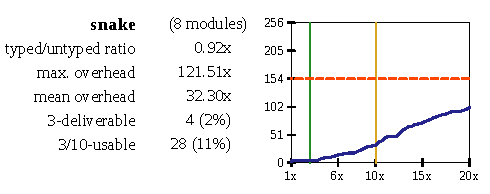
\includegraphics[width=3.5in]{snake} \\
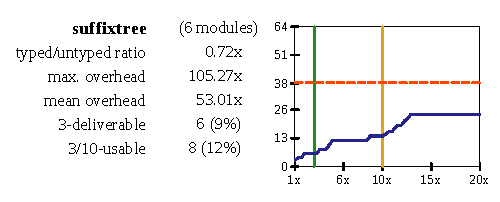
\includegraphics[width=3.5in]{suffixtree}
\end{center}

\footnote{\textit{Is sound gradual typing dead?}
  Takikawa et al. POPL 2016}

}


%===============================================================================
\begin{frame}[fragile]
\frametitle{Casts can cause catastrophic slowdowns}

\begin{center}
\begin{lstlisting}
(define sort!
  : ((Vectorof Dyn) Int Int -> ())
  (lambda ([v : (Vectorof Int)]
       [lo : Int][hi : Int])
    (when (< lo hi)
      (let ([pivot : Int (partition! v lo hi)])
        (sort! v lo (- pivot 1))
        (sort! v (+ pivot 1) hi)))))
\end{lstlisting}
\end{center}

\end{frame}

%===============================================================================
\frame{
\frametitle{Casts can cause catastrophic slowdowns}

\begin{center}
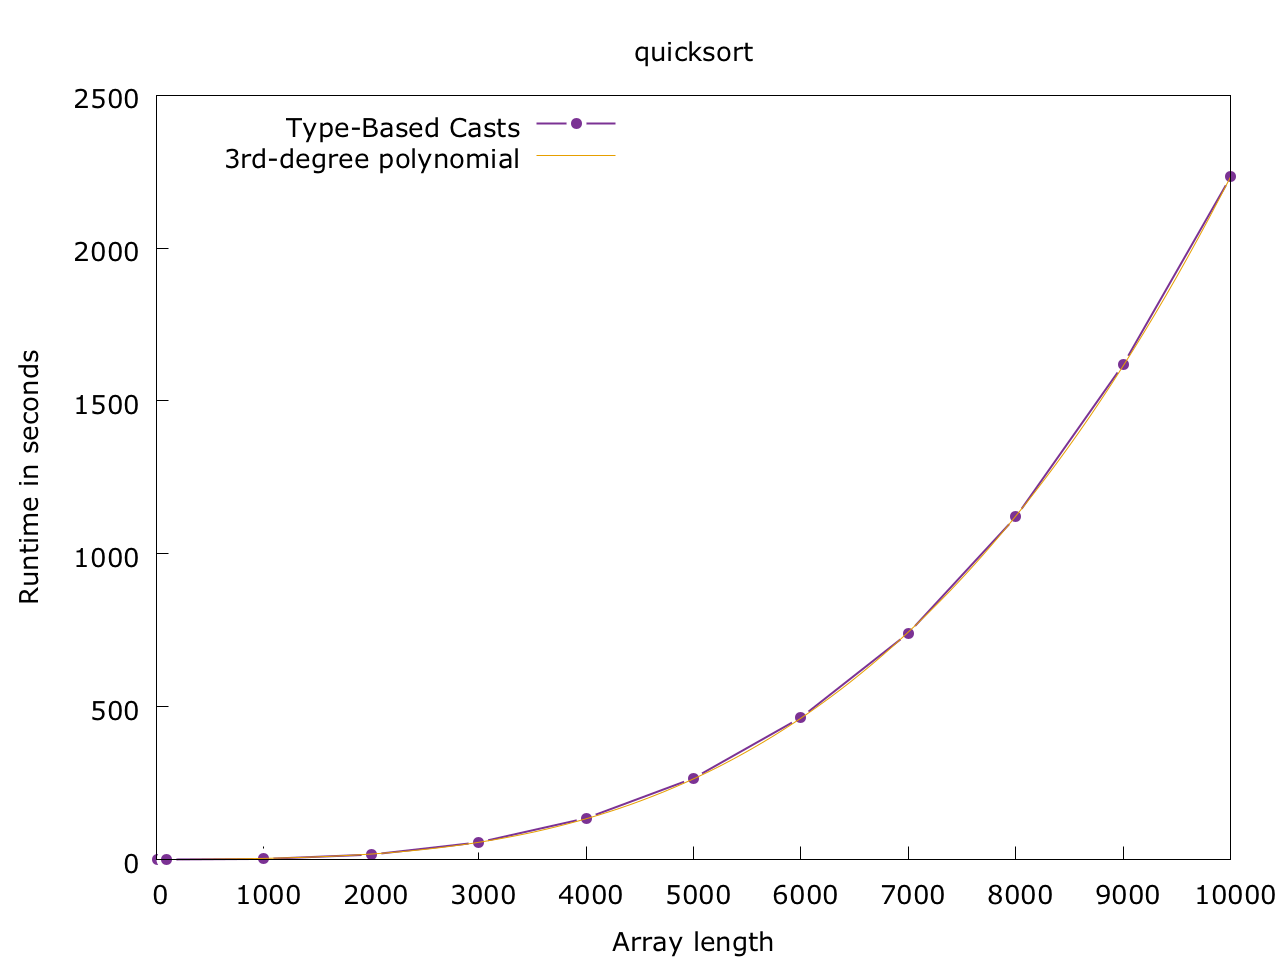
\includegraphics[width=3.5in]{plots/space/quicksort/Type-Based_Casts/poly3fitting.png} \\
\end{center}

}
% ===============================================================================
\frame{
\frametitle{Casts can cause catastrophic slowdowns}

\begin{center}
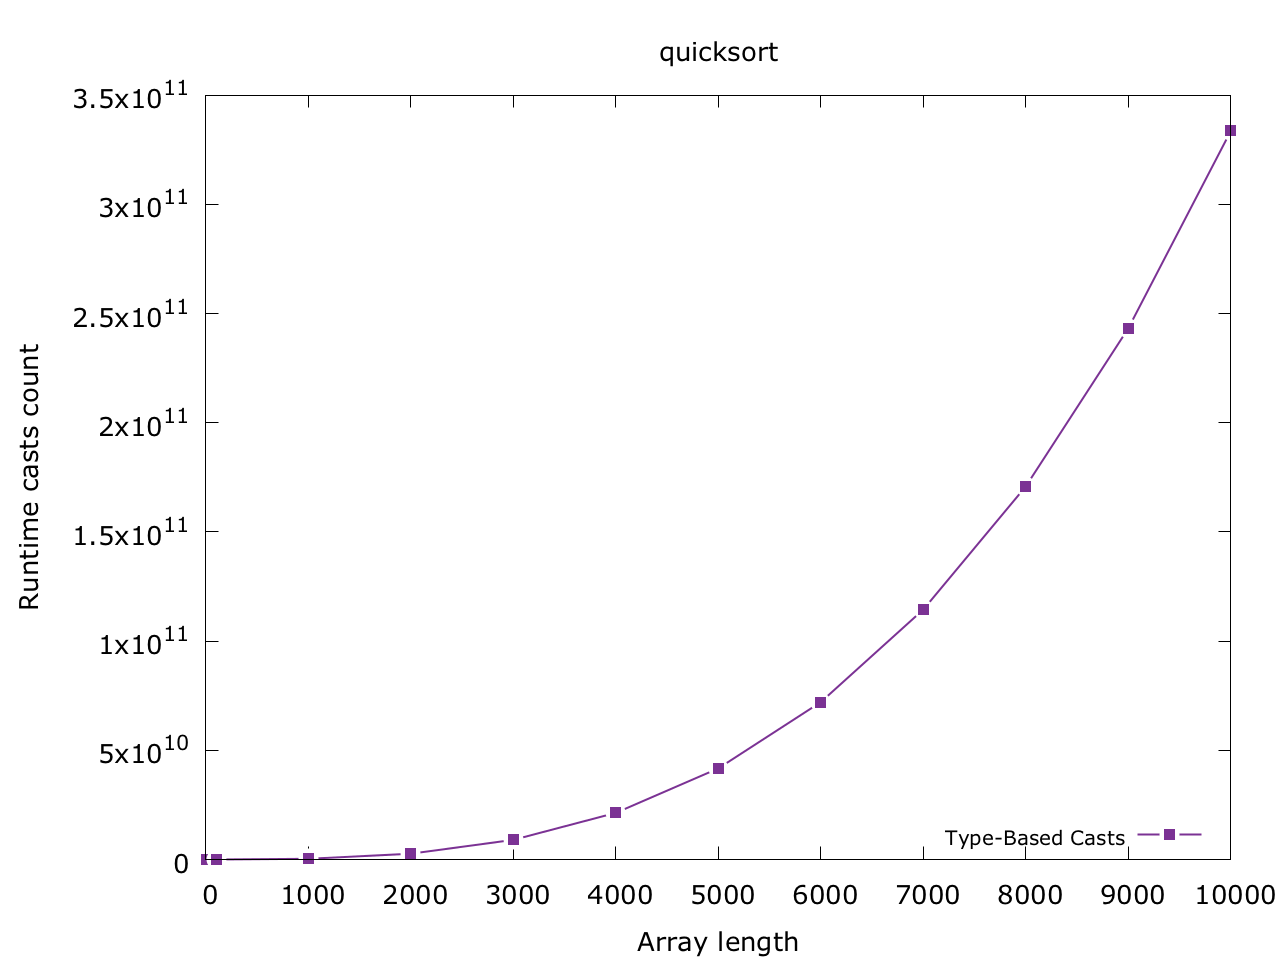
\includegraphics[width=3.5in]{plots/space/quicksort/Type-Based_Casts/casts.png} \\
\end{center}

}
% ===============================================================================
\frame{
\frametitle{Casts can cause long proxy chains}

\begin{center}
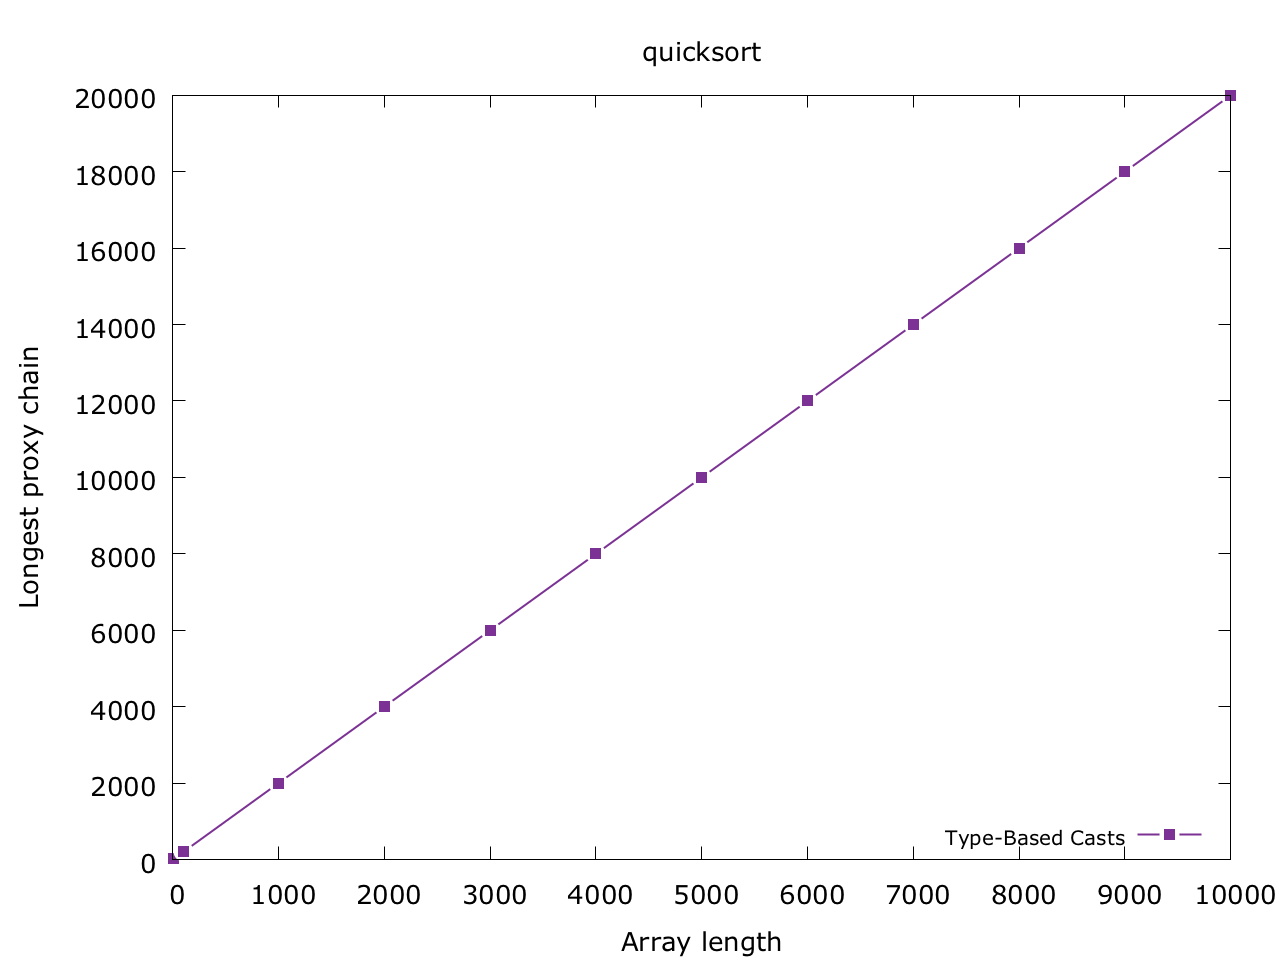
\includegraphics[width=3.5in]{plots/space/quicksort/Type-Based_Casts/lpc.png} \\
\end{center}

}

% ===============================================================================
\frame{
\frametitle{Efficient gradual typing}

\begin{itemize}
\item Challenges to Efficiency
\item \textbf{Challenges to Evaluation}
\item Space-efficient Coercions
\item Monotonic Coercions
\item Performance Comparison
\end{itemize}

}

% ===============================================================================
\frame{
\frametitle{Challenges to Performance Evaluation}

\begin{itemize}
\item Takikawa et al. POPL 2016 proposes to run all the combinations of
  making each module typed or untyped. There are $2^n$
  configurations for a program that consists of $n$ modules.
  \item This should work for most benchmarks where $n$ is relatively
    small.
    \pause
  \item But what if the language supports fine-grained gradual
    typing, where the programmer may opt to not write some type
    annotations or put Dyn inside some?
    \pause
  \item The size of the configuration space for a textbook quicksort is
    248832000000. For n-body, it is
    6914086267191872901144038355222134784.
\end{itemize}

}

%===============================================================================
\frame{
\frametitle{Grift: an experimental compiler}
\begin{itemize}
\item An ahead-of-time optimizing compiler for gradual typing.
\item The source is a functional language with tuples and mutable
  vectors and references, and the target is C.
\item The runtime system implements \textbf{coercions} and
  \textbf{monotonic references}.
\item The compiler specializes casts when their source and/or target
  type is known at compile time.
\item The compiler defers coercion creation until it is actually needed.
\end{itemize}
}

% ===============================================================================

\frame{
\frametitle{Grift Performance Evaluation}

\begin{itemize}
\item a number of configurations are sampled from across the spectrum of
  type precision.
\item Grift is compared on partially typed code to a variant of Grift
  where it is statically typed and does not support gradual typing
  (Static Grift) and to Grift on fully untyped code (Dynamic Grift)
\item Grift is compared on fully typed benchmarks to fully typed
  languages.
\item Grift is compared on fully untyped benchmarks to dynamically typed
  languages.
\end{itemize}

}
% ===============================================================================

\frame{
\frametitle{Efficient gradual typing}

\begin{itemize}
\item Challenges to Efficiency
\item Challenges to Evaluation
\item \textbf{Space-efficient Coercions}
\item Monotonic Coercions
\item Performance Comparison
\end{itemize}

}
% ===============================================================================

\frame{
\frametitle{Compress casts via coercion reduction}

\[
\begin{stack}
\mathit{odd}(0) : \Bool \cast{} \dyn \cast{\ell} \Bool \cast{} \dyn \cast{m} \Bool \cast{} \dyn \\
\\
\mathit{odd}(0) \rd{\CAST{ \pl{\Bool}} \CAST{\qu{\ell}{\Bool}} } \CAST{\pl{\Bool}} \CAST{\qu{m}{\Bool}} \CAST{ \pl{\Bool}}  \\
 \longrightarrow \\
\mathit{odd}(0) \rd{\CAST{\Id{\Bool}} \CAST{ \pl{\Bool}}} \CAST{\qu{m}{\Bool}} \CAST{ \pl{\Bool}}  \\
 \longrightarrow \\
\mathit{odd}(0) \rd{\CAST{ \pl{\Bool}} \CAST{\qu{m}{\Bool}}} \CAST{ \pl{\Bool}}  \\
 \longrightarrow \\
\mathit{odd}(0) \rd{\CAST{\Id{\Bool}} \CAST{ \pl{\Bool}} } \\
 \longrightarrow \\
\mathit{odd}(0) \rd{\CAST{\pl{\Bool}}}
\end{stack}
\]

}
%===============================================================================
\frame{
\frametitle{Coercion Calculus}

%% Blame paths
%% \[
%% p,q ::= \ell \mid p d \mid p r \mid p! \mid p?
%% \]

Syntax
\[
 c,d ::= 
  \Id{T} \mid \pl{I} \mid \qu{\ell}{I} \mid c \to d \mid c \semi d
     \mid \Fail{\ell}
\]
Reduction
\begin{align*}
c ; \Id{T} & \longrightarrow c \\
\Id{T}; c & \longrightarrow c \\
\pl{I} ; \qu{\ell}{I} & \longrightarrow \Id{I}  \\
\pl{I} ; \qu{\ell}{I'} & \longrightarrow \Fail{\ell} & I \neq I' \\
(c \tu d) ; (c' \tu d') & \longrightarrow (c';c) \to (d;d') \\
(\Id{T} \to \Id{T'}) & \longrightarrow \Id{T \to T'} \\
\Fail{\ell}; c & \longrightarrow \Fail{\ell} \\
c;\Fail{\ell} & \longrightarrow \Fail{\ell} &
 \text{if } c \neq \qu{\ell'}{I}
\end{align*}


\footnote{\textit{Dynamic Typing.} Henglein. ESOP 1992}
%\footnote{\textit{Blame and coercion.} Siek, Thiemann, Wadler. PLDI 2015.}
}

%===============================================================================
\frame{
\frametitle{Normalize adjacent coercions}

\begin{align*}
  e &::= \cdots \mid e \CAST{c} & \text{Terms}\\
  u & ::= n \mid \lam{x \of T}e
  & \text{Uncoerced Values} \\
  v & ::=
   u \mid u \CAST{c \tu d} \mid u \CAST{ \pl{I} } 
  & \text{Values}
  %% \EE & ::=  
  %%  \FF \mid \FF[\Hole \CAST{c}] 
  %% & \text{Evaluation contexts}\\
  %% \FF & ::= 
  %%  \Hole \mid \EE[\Hole \app e] \mid \EE[v \app \Hole]
  %% &\text{Cast-free contexts}
\end{align*}
\begin{align*}
  (u \CAST{c \tu d}) \app v
    & \reduce (u \app v \CAST{c}) \CAST{d} \\
    % \label{WrapT}\tagsc{Wrap} \\
  u \CAST{\Id{T}}
    & \reduce u \\
  \rd{e \CAST{c} \CAST{d}}
    & \rd{\reduce e \CAST{c'}} & \text{if } (c;d) \longrightarrow^{*}c'\\
    % \label{ComposeT}\tagsc{Compose} \\
  u \CAST{\bot^\ell}
    & \reduce \blame{\ell}  
\end{align*}
\footnote{\textit{Space-Efficient Gradual Typing.}
  Herman, Tomb, Flanagan. TFP 2006.}
}

%===============================================================================
\frame{
\frametitle{Coercions in normal form \& composition}
\small

\[
\begin{stack}
  % \text{Threesome coercions}
  s,t ::=
   \Id{\dyn} \mid (\qu{\ell}{I} \semi i) \mid i \\
  % \text{Injection coercions}
  i ::= 
   (g \semi \pl{I}) \mid g \mid \FAIL{I}{\ell}{H} \qquad\qquad
  % \text{Ground coercions}
  g,h ::= 
   \Id{\Int} \mid (s \to t) 
\end{stack}
\]
 \hfill \fbox{$s \fatsemi t = s$}
\vspace{-10pt}
\begin{align*}
  \Id{\Int} \fatsemi t = \Id{\dyn} \fatsemi t & = t \\
  (s \to t) \fatsemi (s' \to t') & = (s' \fatsemi s) \to (t \fatsemi t') \span \\
  (g \semi \pl{I}) \fatsemi \Id{\dyn} & = g \semi \pl{I} \\
  (\qu{\ell}{I} \semi i) \fatsemi t & = \qu{\ell}{I} \semi (i \fatsemi t)  \\
  g \fatsemi (h \semi \pl{I}) & = (g \fatsemi h) \semi \pl{I}  \\
  (g \semi \pl{I}) \fatsemi (\qu{\ell}{I} \semi i) & = g \fatsemi i \\
  (g \semi \pl{I}) \fatsemi (\qu{\ell}{I'} \semi i) & = \FAIL{I}{\ell}{I'}
    & \text{if $I \neq I'$} \\
  \FAIL{I}{\ell}{I'} \fatsemi s  = 
  g \fatsemi \FAIL{I}{\ell}{I'} & = \FAIL{I}{\ell}{I'}
\end{align*}
\[
 \FF[e \CAST{s} \CAST{t}]
    \reduce \FF[e \CAST{s \fatsemi t}]
\]
\footnote{\textit{Blame and coercion $\ldots$} Siek, Thiemann, Wadler. PLDI 2015.}
}
%===============================================================================
\frame{
\frametitle{Coercions eliminate catastrophic slowdowns}

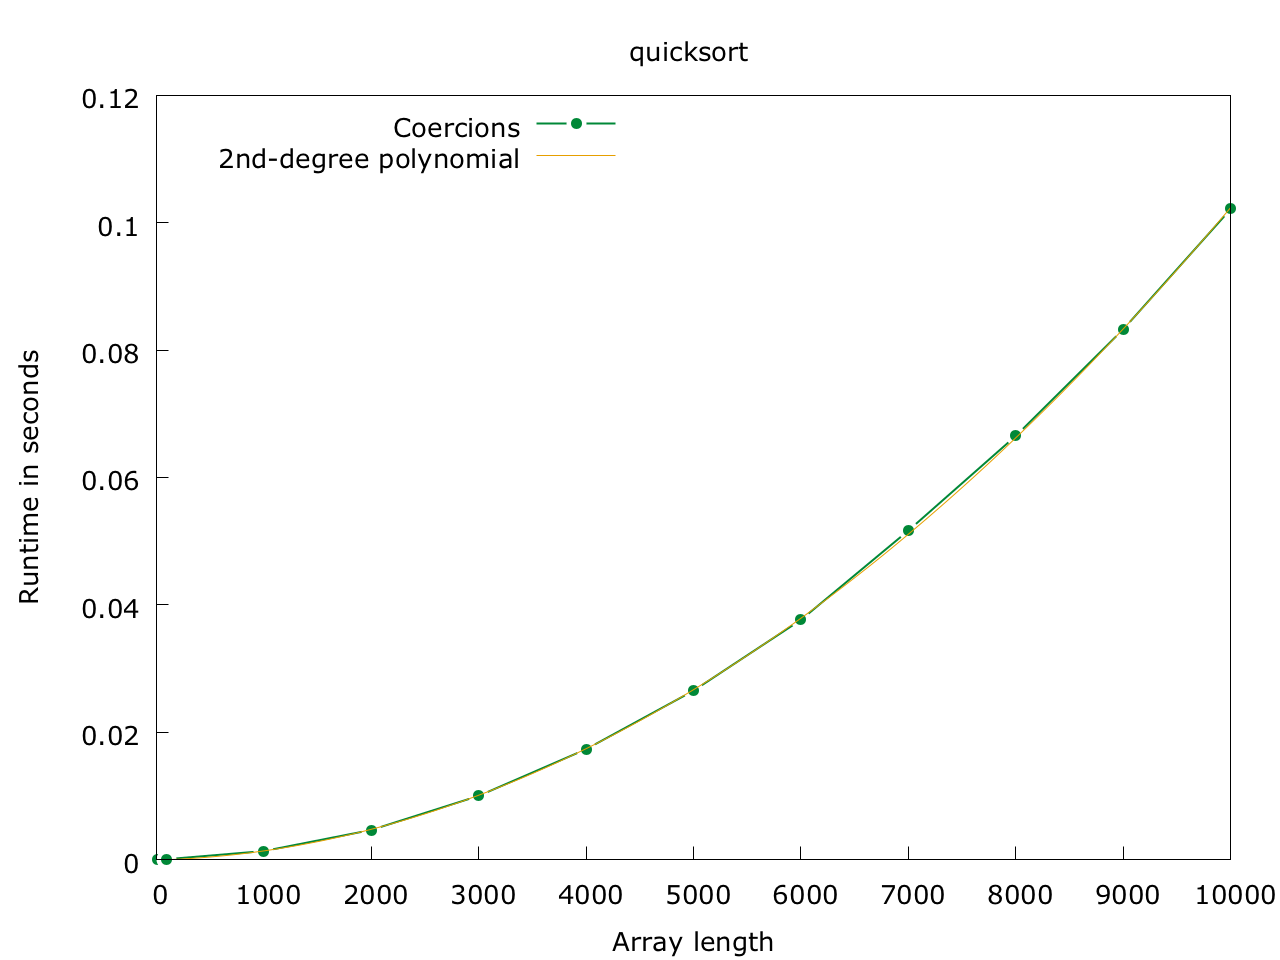
\includegraphics[width=4in]{plots/space/quicksort/Coercions/poly2fitting.png}

}
% ===============================================================================
\frame{
\frametitle{Coercions eliminate catastrophic slowdowns}

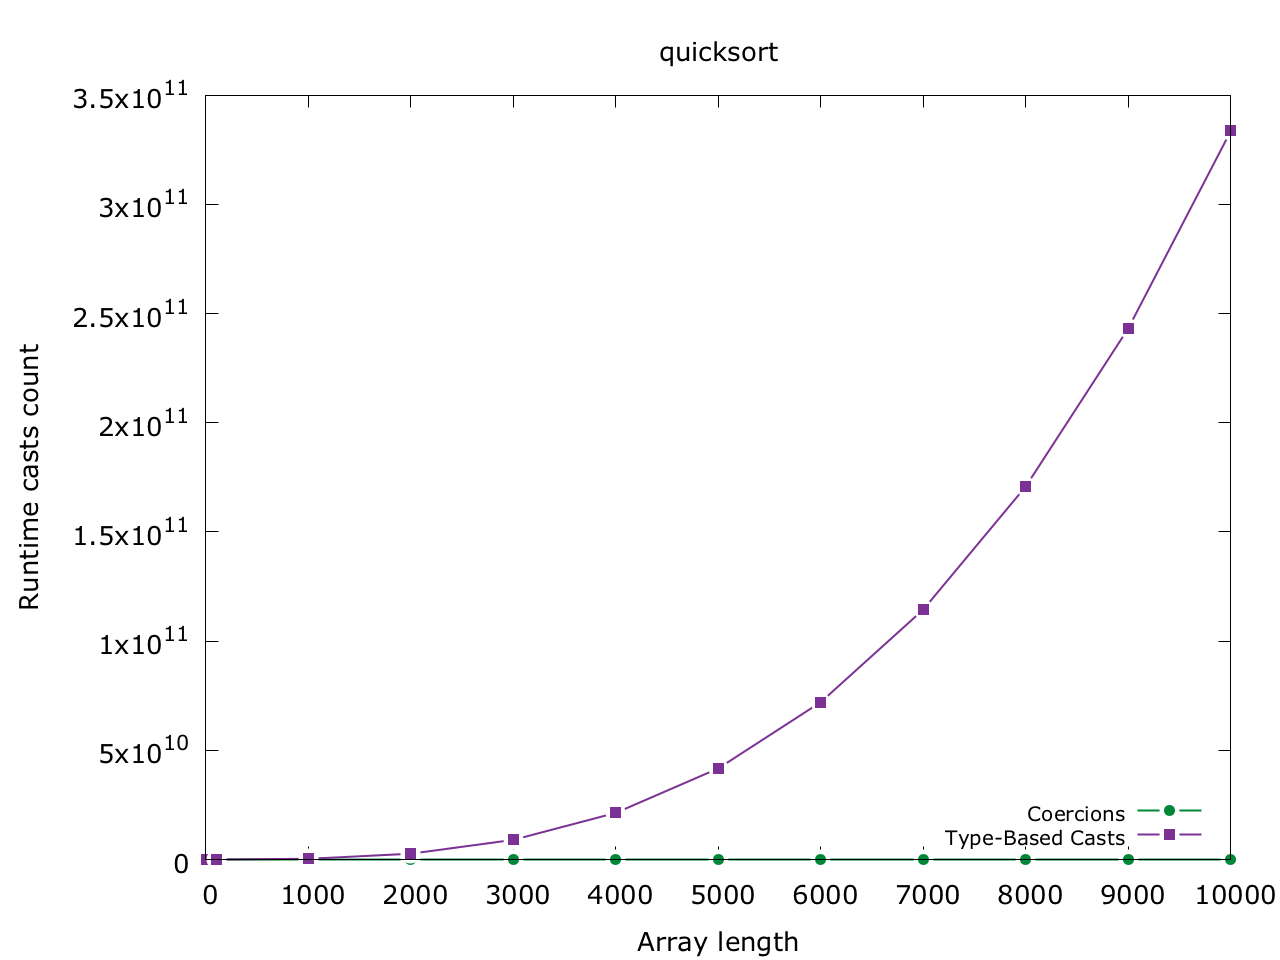
\includegraphics[width=4in]{plots/space/quicksort/casts.png}

}
% ===============================================================================
\frame{
\frametitle{Coercions eliminate catastrophic slowdowns}

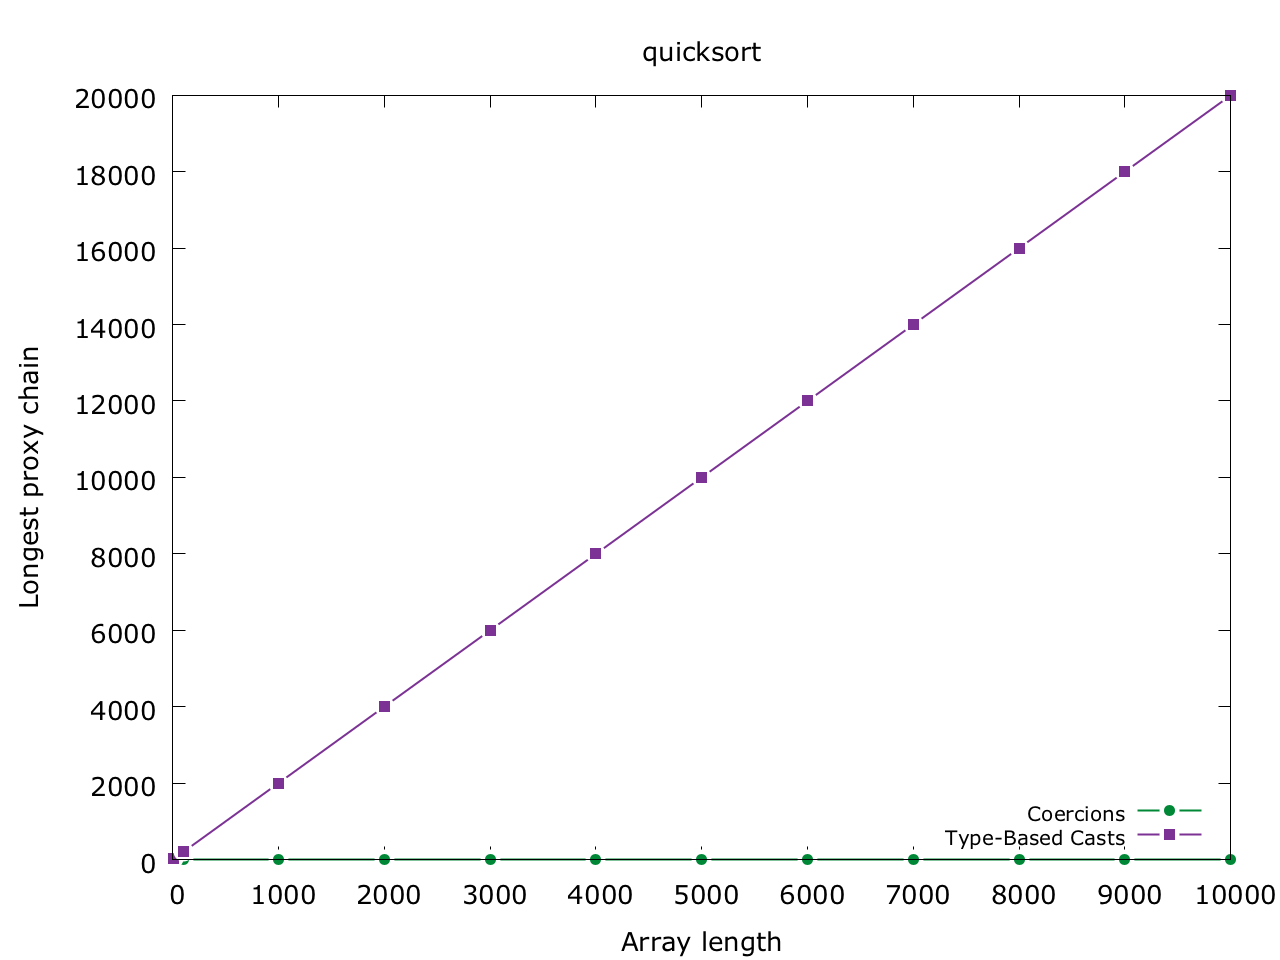
\includegraphics[width=4in]{plots/space/quicksort/lpc.png}

}
% ===============================================================================
\frame{
\frametitle{Coercions eliminate catastrophic slowdowns}

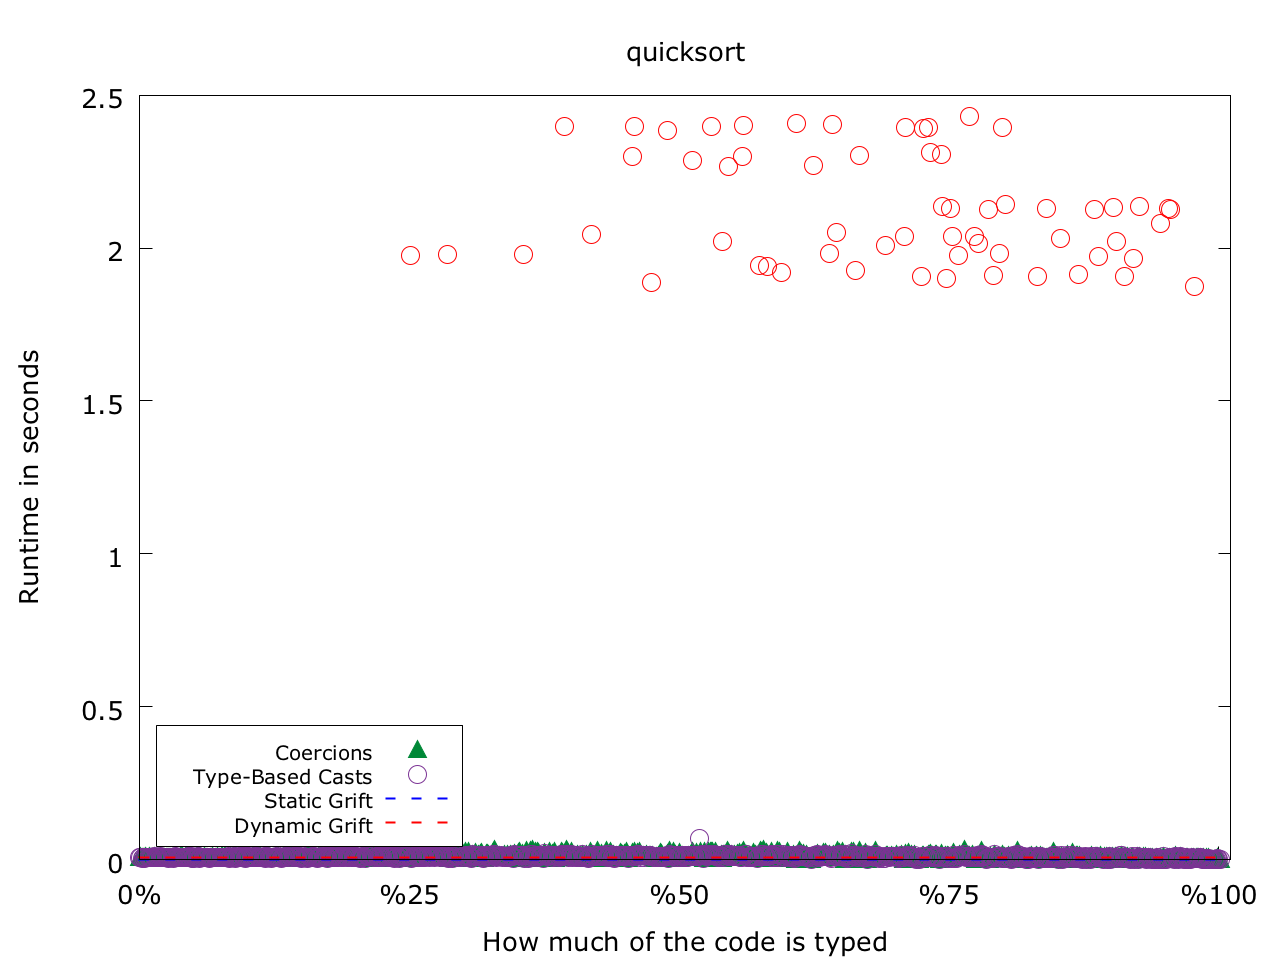
\includegraphics[width=4in]{plots/casts-or-coercions/quicksort/rt.png}
\begin{itemize}
  \item mean speedup of $\kw{13}$ and max speedup of $\kw{1756}$
\end{itemize}
}
%===============================================================================
\frame{
\frametitle{Coercions sometimes incur overhead}

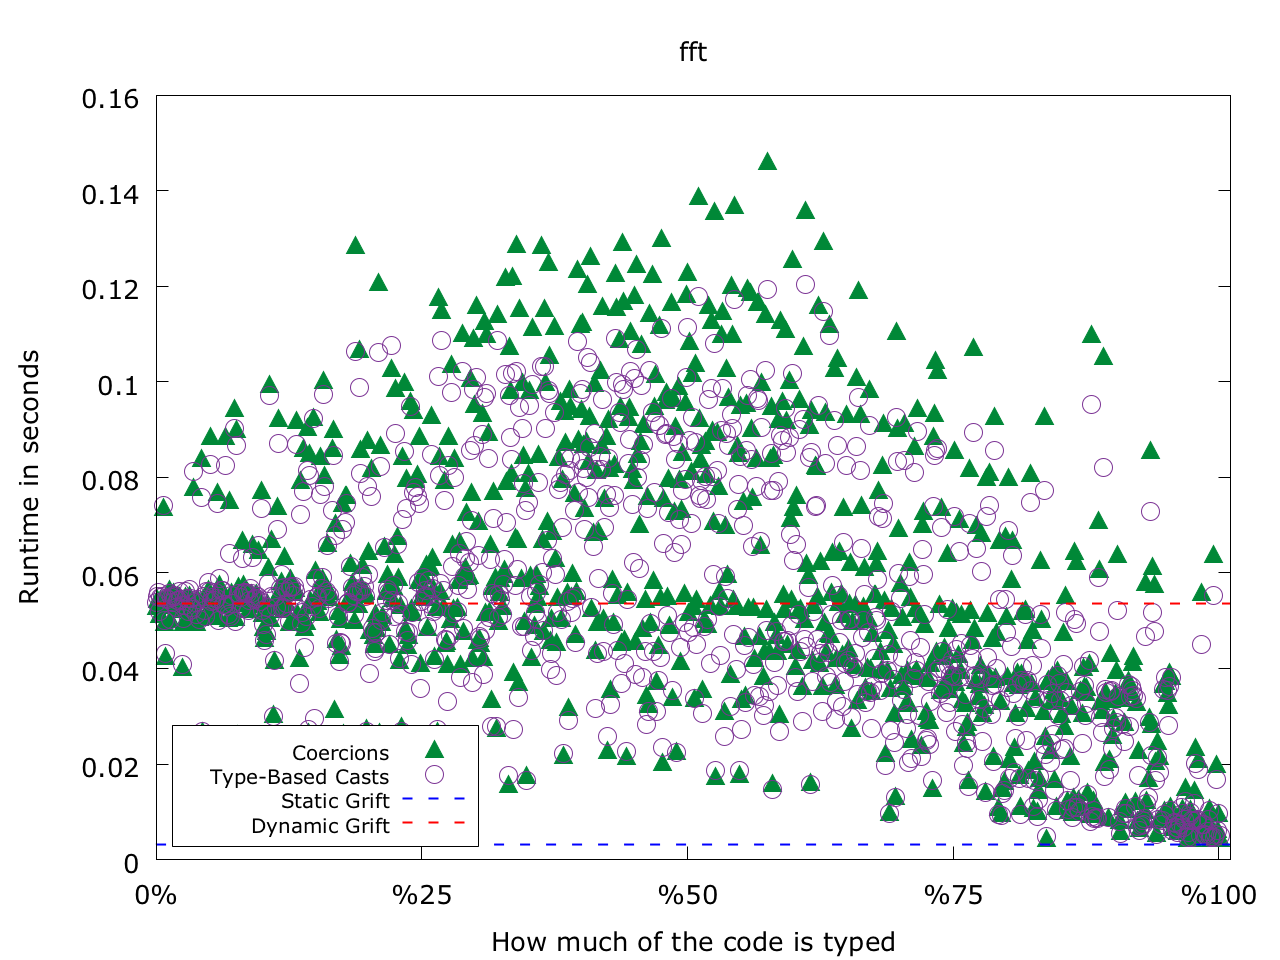
\includegraphics[width=4in]{plots/casts-or-coercions/fft/rt.png}
\begin{itemize}
  \item mean slowdown of $\kw{1.1}$ and max slowdown of $\kw{1.6}$
\end{itemize}

}
%===============================================================================
\frame{
\frametitle{Coercions sometimes pay for themselves}

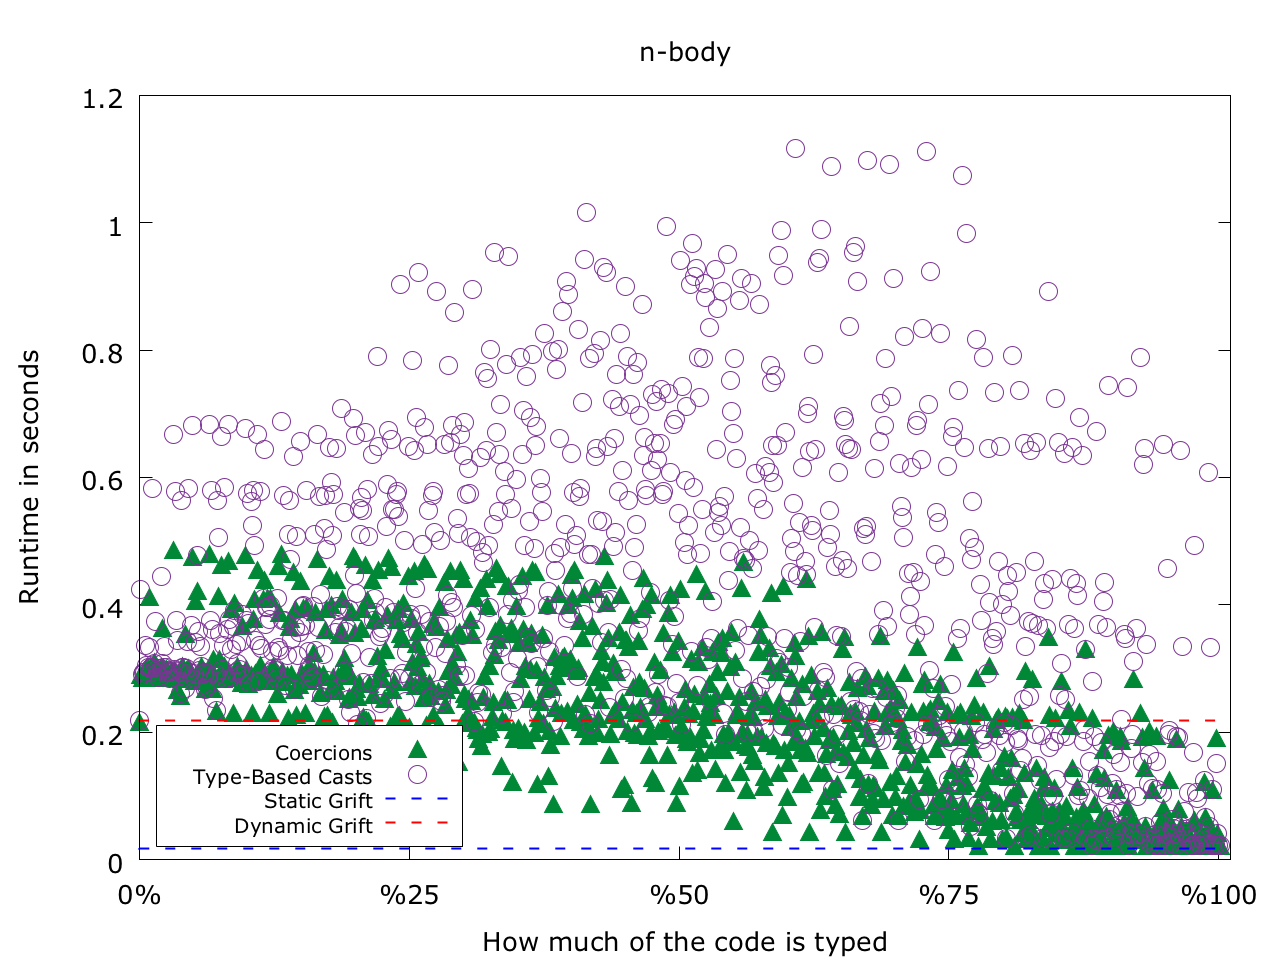
\includegraphics[width=4in]{plots/casts-or-coercions/n_body/rt.png}
\begin{itemize}
  \item mean speedup of $\kw{1.9}$ and max speedup of $\kw{28}$
\end{itemize}

}
% ===============================================================================

\frame{
\frametitle{Coercions sometimes pay for themselves}

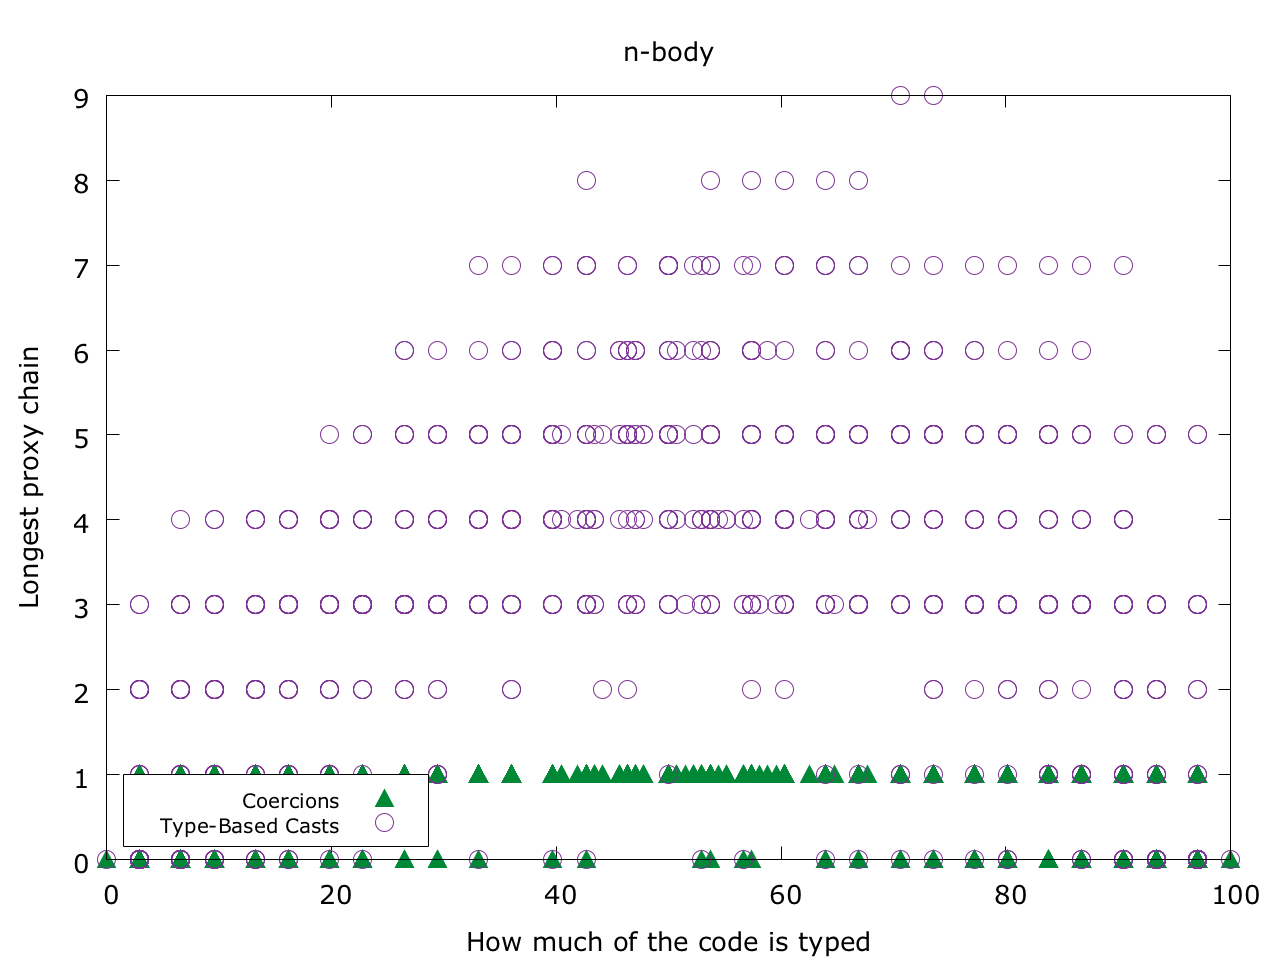
\includegraphics[width=4in]{plots/casts-or-coercions/n_body/lpc.png}

}
%===============================================================================
\frame{
\frametitle{Efficient gradual typing}

\begin{itemize}
\item Challenges to Efficiency
\item Challenges to Evaluation
\item Space-efficient Coercions
\item \textbf{Monotonic Coercions}
\item Performance Comparison
\end{itemize}

}
%===============================================================================
\frame{
\frametitle{Gradual typing with mutable references}
\vspace{5pt}
\begin{align*}
  T & ::= \cdots \mid \Ref T \\
  e & ::= \cdots \mid \alloc e \mid \deref^\ell e \mid e \update^\ell e \\
  v & ::= \cdots \mid a \mid a \CAST{\Ref (c,d)}
\end{align*}
Consistency \hfill \fbox{$T \sim T$}
\[
\cdots
\qquad
\inference
  {T_1 \sim T_2}
  {\Ref T_1 \sim \Ref T_2}
\]

Coercions
\[
c ::= \ldots \mid \Ref(c_1, c_2)
\]

Compile Casts to Coercions
\begin{align*}
  \bcfun{\Ref T_1 \cast{\ell} \Ref T_2}
    &=  \Ref(\bcfun{T_1 \cast{\ell} T_2}, \bcfun{T_2 \cast{\ell} T_1})
\end{align*}

\footnote{\textit{Space-Efficient Gradual Typing.}
  Herman, Tomb, Flanagan. TFP 2006.}

}
%===============================================================================
\frame[containsverbatim]{
\frametitle{Example of overhead in reference access}

\begin{minipage}{0.6\textwidth}
\begin{lstlisting}
fun f(p3:Ref Int, p4:Ref Int)=
    !p3 + !p4;
\end{lstlisting}
\hrule
\begin{lstlisting}
val p1 = ref 5;
val p2 = ref (6|<Int!>|);

f(p1, p2|<Ref(Int?,Int!)>|);


|ref(Int?,Int!)| 
  : Ref $\dyn$ $\Rightarrow$ Ref Int
\end{lstlisting}
\end{minipage}
\vrule
\begin{minipage}{0.38\textwidth}
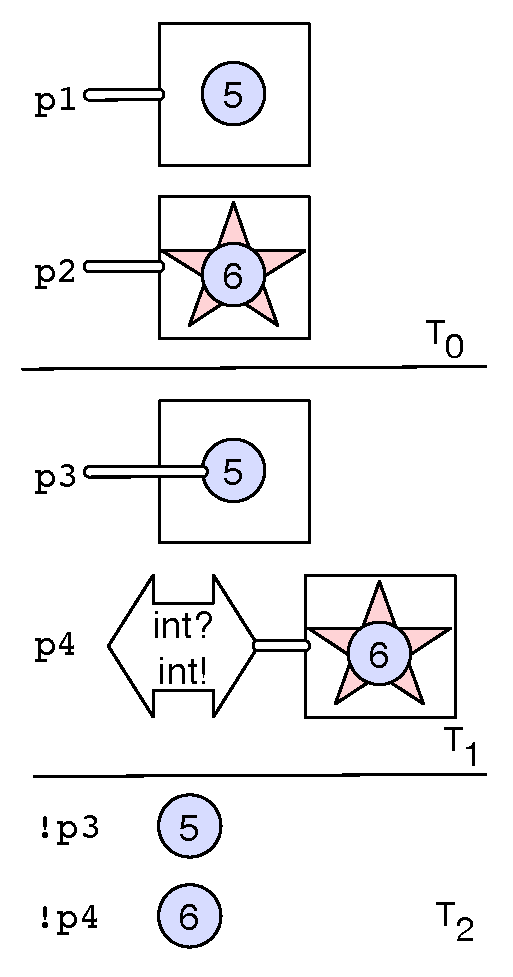
\includegraphics[height=2.65in]{HermanRefCoerce}
\end{minipage}

\fbox{
\begin{minipage}{\textwidth}
Problem: generated code for \lstinline{!p3} and \lstinline{!p4}
must branch at runtime for the two kinds of references.
\end{minipage}
}

}
%===============================================================================
\frame{
\frametitle{Root of the problem}

\begin{theorem}[Canonical Forms]
Suppose $\emptyset \vdash v : T$. If $T=\Ref T$, then either
\begin{itemize}
\item $v = a\;$ for some address $a$, or
\item $v = a \CAST{\Ref(c_1, c_2)}$.
\end{itemize}
\end{theorem}

Two rules for dereference
\begin{align*}
\deref a, \mu & \reduce \mu(a), \mu  \\
\deref (a\CAST{\Ref(c_1, c_2)}),\mu & 
    \reduce (\deref a)\CAST{c_1} , \mu\\
\end{align*}
Two rules for update
\begin{align*}
a \update v, \mu & \reduce a, \mu(a \mapsto v) \\
a \CAST{\Ref(c_1,c_2)} \update v, \mu  & 
    \reduce a \update v \CAST{c_2} , \mu
\end{align*}

}
%===============================================================================
\frame[containsverbatim]{
\frametitle{Monotonic References}

\begin{minipage}{0.6\textwidth}
\begin{lstlisting}
fun f(p3:Ref Int, p4:Ref Int)=
    !p3 + !p4;
\end{lstlisting}
\hrule
\begin{lstlisting}
val p1 = ref 5;
val p2 = ref (6|<Int!>|);

f(p1, p2|<Ref(Int)>|);



$ $
\end{lstlisting}
\end{minipage}
\vrule
\begin{minipage}{0.38\textwidth}
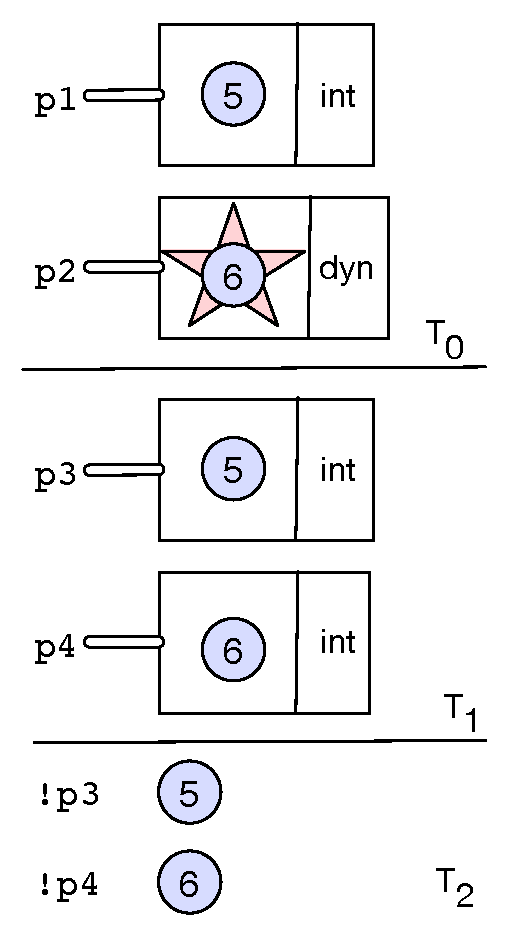
\includegraphics[height=2.6in]{MonoRefCoerce}
\end{minipage}
\fbox{
\begin{minipage}{\textwidth}
Update the reference cell to the \emph{meet} of the
current RTTI and the target of the cast.
\end{minipage}
}

\footnote{\textit{Monotonic Ref. for Efficient Gradual Typing.}
  Siek et al. ESOP 2015}

}
%===============================================================================

\frame[containsverbatim]{
\frametitle{Aliasing and Static vs. Dynamic Dereference}

\vspace{10pt}

\begin{minipage}{0.6\textwidth}
\begin{lstlisting}
fun f(x:Ref Int, y:Ref $\dyn$)=
    ~!x~ + |!y@$\rd{\dyn}$|;

p = ref (2|<Int!>|);
f(p, p);
\end{lstlisting}
\end{minipage}
\vrule
\quad
\begin{minipage}{0.35\textwidth}
Compile-time choice:
\begin{itemize}
\item {\color{blue} Fast static deref.}
\item {\color{red} Slow dynamic dereference}
\end{itemize}
\end{minipage}

\begin{center}
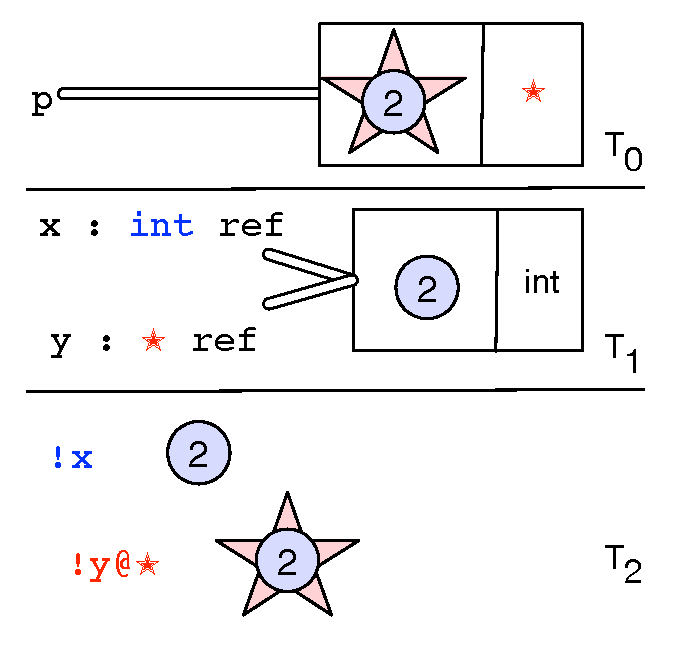
\includegraphics[height=2in]{MonoAlias}
\end{center}
}


%===============================================================================

\frame{
\frametitle{The Monotonic Invariant}

\begin{minipage}{0.8\textwidth}
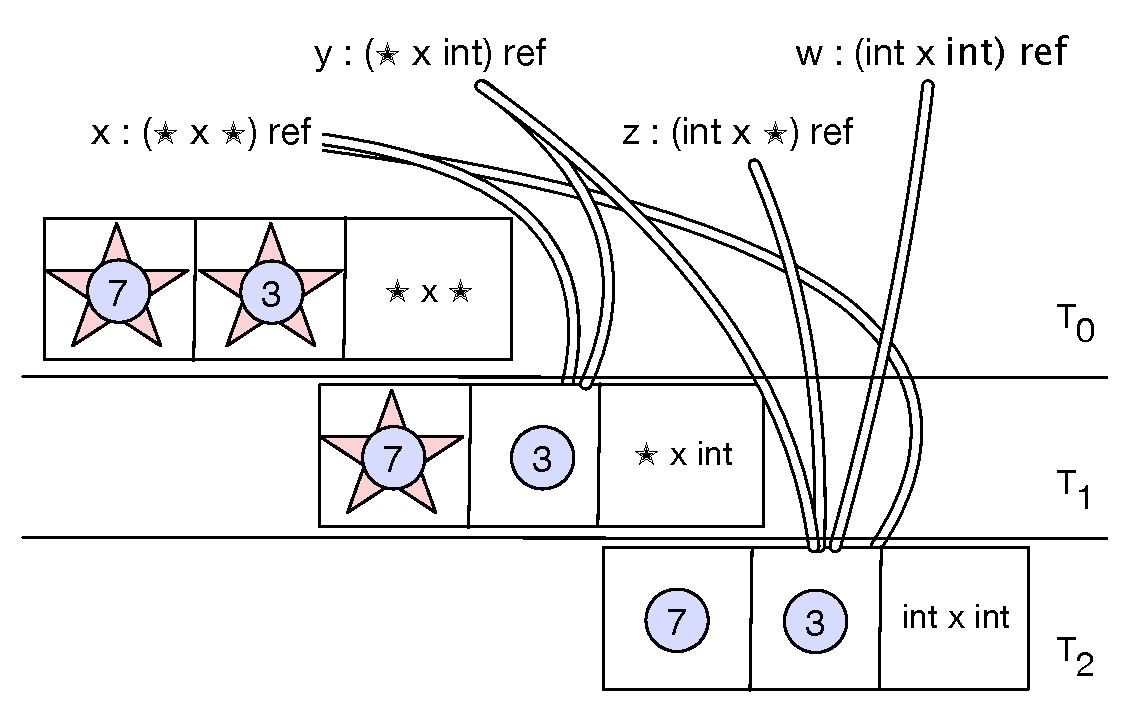
\includegraphics[height=2in]{MonoInvariant}
\end{minipage}
\begin{minipage}{0.2\textwidth}
\xymatrix{
  \Dyn \times \Dyn  \ar[d]^{\sqsubseteq}\\
  \Dyn \times \Int \ar[d]^{\sqsubseteq} \\
  \Int \times \Int
}
\end{minipage}

\fbox{
\begin{minipage}{\textwidth}
\begin{itemize}
\item The RTTI of a cell may become more precise. 
\item Every reference is less or equally precise as the RTTI. 
\item If a reference is fully static (e.g. w), then so is the cell.
\end{itemize}
\end{minipage}
}

}

%% %===============================================================================
%% \frame{
%% \frametitle{Reduction Rules for Casting References}

%% Casting References\hfill $\mu(a)=cv:T_1$
%% \begin{gather*}
%% \inference{T_3 = T_1 \MergeT T_2 &
%%            T_3 \neq T_1}
%%           {a \CAST{\RefC{T_2}},\mu \longrightarrow a, \mu(a \mapsto (cv \CAST{\llbracket T_1 {\To} T_3 \rrbracket}): T_3)  } \\[2ex]
%% \inference{T_3 = T_1 \MergeT T_2 & T_3 = T_1}
%%           {a \CAST{\RefC{T_2}},\mu \longrightarrow a, \mu} \\[2ex]
%% \inference{T_1 \MergeT T_2 = \bot}
%%           {a \CAST{\RefC{T_2}},\mu \longrightarrow \error, \mu}
%% \end{gather*}

%% }
%% %===============================================================================
%% \frame{
%% \frametitle{Reduction Rules for Accessing References}

%% Deference \hfill $\mu(a) = v : T$
%% \begin{align*}
%% \color{blue}\deref a, \mu & \color{blue}\longrightarrow v, \mu  \\
%% \color{red}\deref a @ T', \mu & \color{red} \longrightarrow  v \CAST{\llbracket T \To T' \rrbracket}, \mu
%% \end{align*}
%% Update
%% \begin{align*}
%% \color{blue}a \update v', \mu & \color{blue}\longrightarrow a, \mu(a \mapsto v':T) \\
%% \color{red}a \update v' @ T', \mu & \color{red}\longrightarrow a, \mu(a \mapsto (v' \CAST{\llbracket T' \To T \rrbracket} ) : T) 
%% \end{align*}

%% }
%% %===============================================================================
%% \frame{
%% \frametitle{Reduction Rules for Heap Quiescence}

%% \begin{syntax}
%% \text{Casted Values} & cv & ::= & v \mid cv \CAST{c} \\
%% \text{Heap} & \mu & ::= & \emptyset \mid \mu(a \mapsto v:T) \\
%% \text{Evolving Heap} & \nu & ::= & \emptyset \mid \nu(a \mapsto cv:T)  \\
%% \end{syntax}

%% \begin{gather*}
%% \inference
%%     {\nu(a) = cv:T & cv,\nu \reduce cv',\nu' &
%%      \rtti{\nu'}{a} = T}
%%     {e, \nu \reduce e, \nu'(a \mapsto cv':T) }
%% \\[2ex]
%% \inference
%%     {\nu(a) = cv:T & cv,\nu \reduce cv',\nu' &
%%      \rtti{\nu'}{a} \neq T}
%%     {e, \nu \reduce e, \nu'}
%% \end{gather*}
%% (omitted error handling rules)

%% }
%===============================================================================
\frame{
\frametitle{Monotonic implementation}

\begin{itemize}
\item hashconsing types at runtime to speedup the meet operation
\item casted tuple values are just copies of the original tuples written
  to the heap and updated in place while the cast is in progress.
\end{itemize}

}
%===============================================================================
\frame{
\frametitle{Monotonic eliminates overhead in static code}

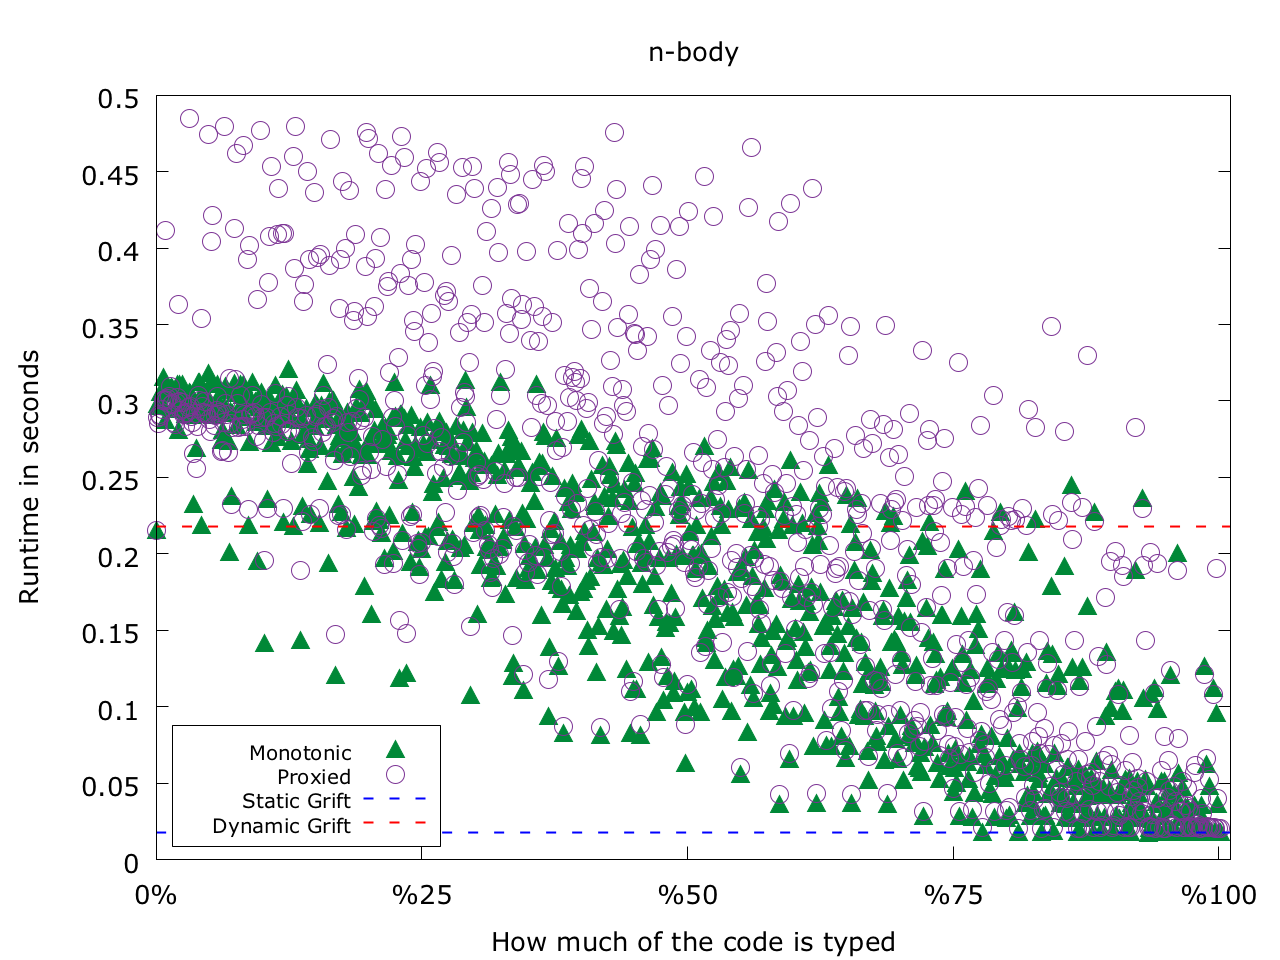
\includegraphics[width=4in]{plots/monotonic-v-coercions/n_body/rt.png}

\begin{itemize}
  \item mean speedup of 1.26 and max speedup of 3.24
\end{itemize}

}
%===============================================================================
\frame{
\frametitle{Montonic doesn't matter for some programs}

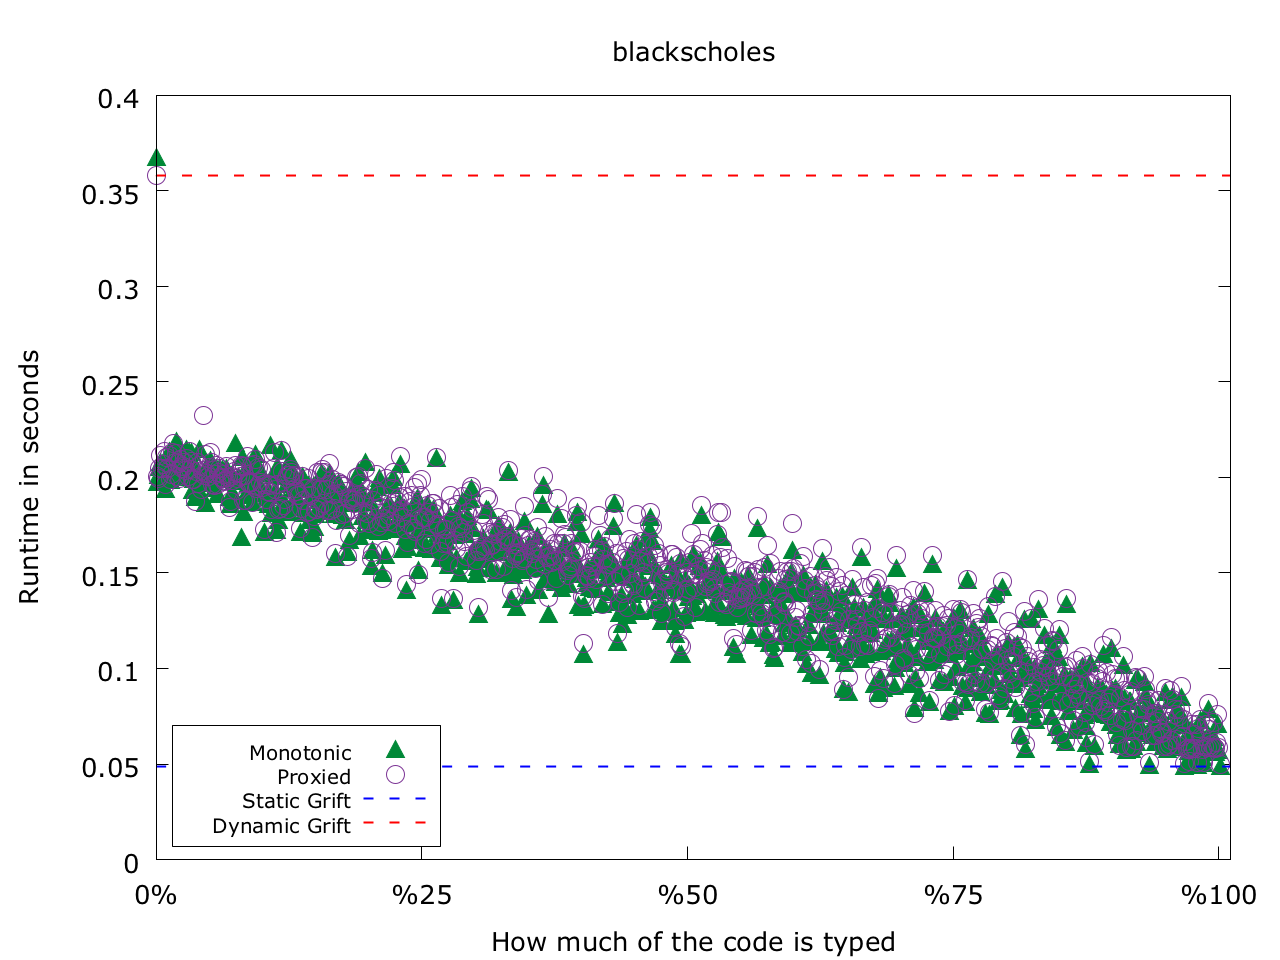
\includegraphics[width=4in]{plots/monotonic-v-coercions/blackscholes/rt.png}

}
%===============================================================================
\frame{
\frametitle{Efficient gradual typing}

\begin{itemize}
\item Challenges to Efficiency
\item Challenges to Evaluation
\item Space-efficient Coercions
\item Monotonic Coercions
\item \textbf{Performance Comparison}
\end{itemize}

}
%===============================================================================


%% to do: specialization

%===============================================================================
\frame{
\frametitle{Comparison on dynamically typed programs}

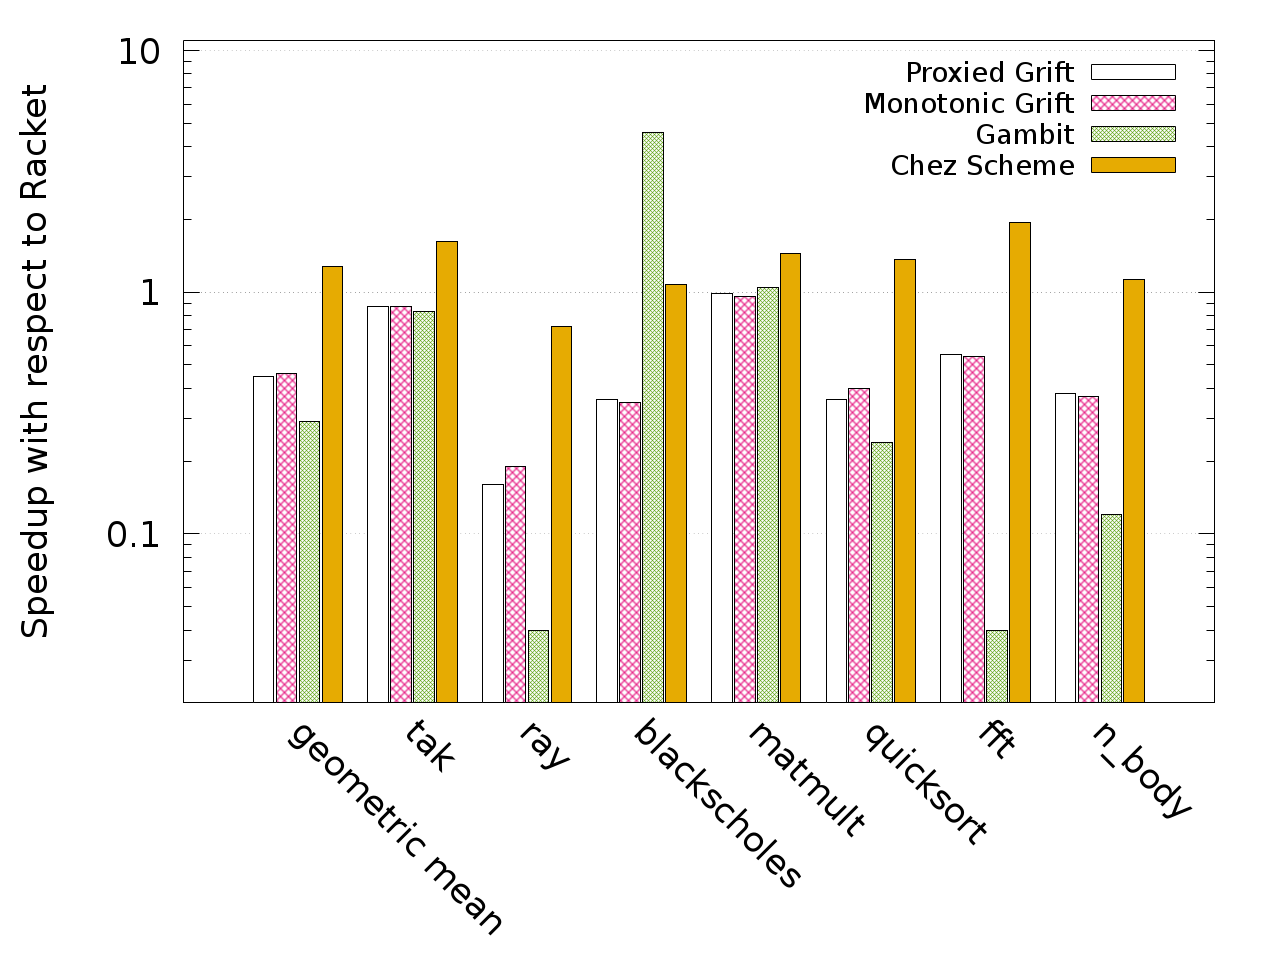
\includegraphics[width=4in]{plots/external/Specialized_Lazy_Coercions_dynamic.png}

}
%===============================================================================
\frame{
\frametitle{Comparison on statically typed programs}

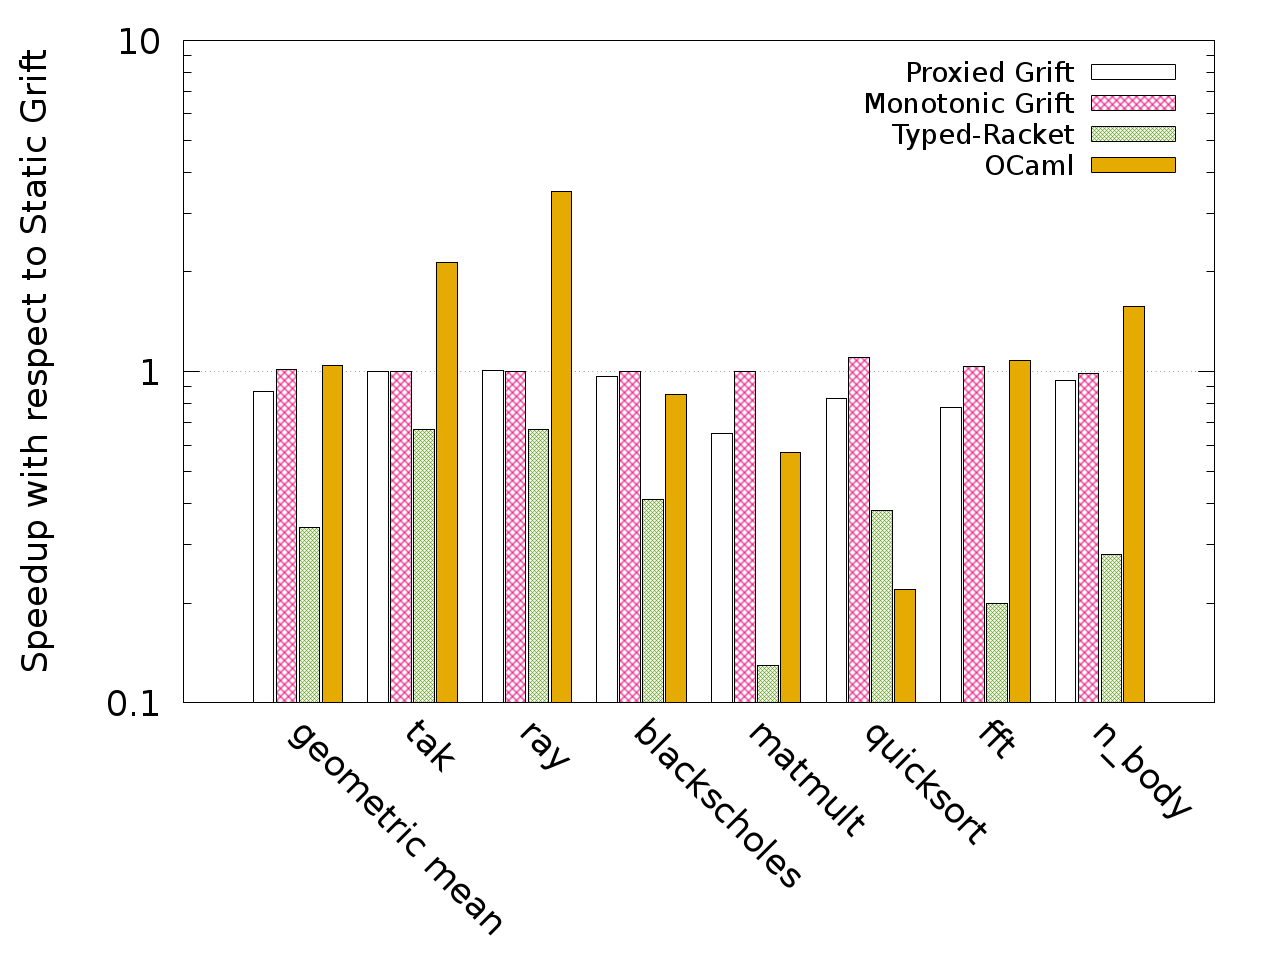
\includegraphics[width=4in]{plots/external/Specialized_Lazy_Coercions_static.png}

}
%===============================================================================
%% \frame{
%% \frametitle{Compose adjacent coercions}

%% %% \begin{align*}
%% %%   u & ::= n \mid \lam{x \of T}e
%% %%   & \text{Uncoerced Values} \\
%% %%   v & ::=
%% %%    u \mid u \CAST{s \to t} \mid u \CAST{g \semi \pl{I}} 
%% %%   & \text{Values}\\
%% %%   \EE & ::=  
%% %%    \FF \mid \FF[\Hole \CAST{s}] 
%% %%   & \text{Evaluation contexts}\\
%% %%   \FF & ::= 
%% %%    \Hole \mid \EE[\Hole \app e] \mid \EE[v \app \Hole]
%% %%   &\text{Cast-free contexts}
%% %% \end{align*}

%% \begin{align*}
%%   %% \EE[(u \CAST{s \to t}) \app v]
%%   %%   & \reduce \EE[(u \app v \CAST{s}) \CAST{t}] \\
%%   %%   % \label{WrapT}\tagsc{Wrap} \\
%%   %% \FF[u \CAST{\Id{}}]
%%   %%   & \reduce \FF[u] \\
%%    % \label{ComposeT}\tagsc{Compose} \\
%%   %% \FF[u \CAST{\FAIL{I}{\ell}{I'}}]
%%   %%   & \reduce \blame{\ell}  \\
%%   %%   % \label{FailT}\tagsc{Fail}
%%   %% \EE[\blame{\ell}]
%%   %%   & \reduce \blame{\ell}
%%   %%   & \text{if $\EE \neq \Hole$}
%% \end{align*}

%% }

%===============================================================================
%% \frame{
%% \frametitle{Stay tuned...}

%% \begin{itemize}
%% \item ... for performance evaluations.

%% \item We are developing a compiler for the GTLC in which to
%%   empirically test these ideas.

%% \item The PLT Racket folks are evaluating and improving the efficiency
%%   of contracts.
%% \end{itemize}

%% \footnote{\textit{Towards absolutely efficient gradually typed languages.}\\
%%   \qquad\qquad Kuhlenschmidt et al. STOP 2015}
%% \footnote{\textit{Towards Practical Gradual Typing.}
%%    Takikawa et al. ECOOP 2015}

%% }
%===============================================================================
\frame{
\frametitle{Conclusion}

\begin{itemize}
\item Gradual typing can be efficient!
\item On dynamically typed code: competative with Gambit.
\item On statically typed code: competative with OCaml.
\item On partially typed code, performance varies roughly between \%50
  of untyped impl. to \%100 of typed impl.
\item Use \textbf{coercions} to eliminate catastrophic slowdowns
  in partially typed code.
\item Use \textbf{monotonic references} to reduce overhead in
  statically typed code.
\end{itemize}


}

%===============================================================================
\frame{
\frametitle{}

\center{Grift is open source: github.com/Gradual-Typing/Grift}
\vspace{0.7in}
\center{\Large Thank you!}


}

\end{document}

%===============================================================================
\frame{
\frametitle{Exercise: Type Ascription}

What is the gradual typing rule for type ascription?
\[
\inference{\Gamma \vdash e : T}
          {\Gamma \vdash e \;\mathsf{as}\; T : T }
\]

\uncover<2->{
Solution
\[
\inference{\Gamma \vdash e : T_1 & T_1 \consis T_2}
          {\Gamma \vdash e \; \mathsf{as}\; T_2 : T_2 }
\]
}

}

%===============================================================================
\frame{
\frametitle{Homework: Sums}

What are the gradually typed versions of the typing rules for disjoint
sums?
\begin{gather*}
\inference{\Gamma \vdash e : T_1}
          {\Gamma \vdash \key{inl} \, e \, \key{as}\, T_1 {+} T_2 : T_1 {+} T_2}
\;
\inference{\Gamma \vdash e : T_2}
          {\Gamma \vdash \key{inr} \, e \, \key{as}\, T_1 {+} T_2 : T_1 {+} T_2}
\\[2ex]
\inference{\Gamma \vdash e_1 : T_1{+}T_2\\
           \Gamma, x:T_1\vdash e_2: T &
           \Gamma, x:T_2\vdash e_3: T}
          {\Gamma \vdash (\case{e_1}{e_2}{e_3}) : T}
\end{gather*}

}
%===============================================================================
%% \frame{
%% \frametitle{Solution}
%% Sums:
%% \[
%% \inference{\Gamma \vdash e_1 : T_4 & T_4 \triangleright T_1{+}T_2\\
%%    \Gamma, x:T_1\vdash e_2: T' &
%%    \Gamma, x:T_2\vdash e_3: T'' & T = \meet{T'}{T''}}
%% {\Gamma \vdash (\case{e_1}{e_2}{e_3}): T}
%% \]

%% Greatest lower bound with respect to the less dynamic (imprecision)
%% relation (e.g., $T \ledyn \dyn$).

%% }

%===============================================================================
\frame{
\frametitle{Compile Casts to Coercions}

\hfill \fbox{$\bcfun{T \cast{\ell} T} = c$}
\begin{align*}
  \bcfun{B \cast{\ell} B}
    &= \Id{B} \\
  \bcfun{T_1 \tu T_2 \cast{\ell} T'_1 \tu T'_2} 
    &= \bcfun{T'_1 \cast{\ell} T_1} \tu \bcfun{T_2 \cast{\ell} T'_2}  \\
  \bcfun{\dyn \cast{\ell} \dyn}
    &= \Id{\dyn} \\
  \bcfun{G \cast{\ell} \dyn}
    &= \pl{I} \\
  \bcfun{T \cast{\ell} \dyn}
    &= \bcfun{T \cast{\ell} G} \semi \pl{I} \qquad \dagger \\
  \bcfun{\dyn \cast{\ell} G}
    &= \qu{\ell}{I} \\
  \bcfun{\dyn \cast{\ell} T}
    &= \qu{\ell}{I} \semi \bcfun{G \cast{\ell} T} \qquad \dagger
\end{align*}
$\dagger$ \ if $T \neq \dyn, T \neq G, T \consis G$

}
%===============================================================================

\frame{
\frametitle{Hyper-coercions, brand new!}
\small

\[
\begin{array}{llcl}
  \text{optional projection} & p & ::= & \epsilon \mid \;?^\ell\\
  \text{opt. inject or fail} & i & ::= & \epsilon \mid \;! \mid \bot^\ell \\
  \text{middle}              & m & ::= & B \mid c {\to} c\\
  \text{hyper-coercions}     & c,d & ::= & \Id{\dyn} \mid \hy{p}{m}{i}
\end{array}
\]
 \hfill \fbox{$c \fatsemi c = c$}
\vspace{-10pt}
\begin{align*}
  \Id{\dyn} \fatsemi c = c \fatsemi \Id{\Dyn} &= c \\
  \hy{p_1}{m_1}{i_1} \;\fatsemi\; \hy{p_2}{m_2}{i_2} &= 
    \hy{p_1}{m_1 \fatsemi m_2}{i_2} & \text{if } m_1 \consis m_2 \\
  \hy{p_1}{m_1}{i_1} \;\fatsemi\; \hy{\,?^\ell}{m_2}{i_2} & = \hy{p_1}{m_1}{\bot^\ell} 
   & \text{if } m_1 \not\consis m_2 \\
  \hy{p}{m}{\bot^\ell} \;\fatsemi\; c &= \hy{p}{m}{\bot^\ell}
\end{align*}
 \hfill 
\[
  B \fatsemi B = B \qquad
  (c {\to} d) \fatsemi (c' {\to} d') = (c' \fatsemi c) \to (d \fatsemi d')
  \qquad
  \fbox{$m \fatsemi m = m$}
\]
\qquad $B \consis B \qquad\qquad c {\to} d \consis c' {\to} d'$
\hfill \fbox{$m \consis m$}


\footnote{Inspired by: Calculating Threesomes. Garcia, ICFP 2013.}
}
%===============================================================================
\frame{
\frametitle{Normalize Adjacent Coercions}

\begin{align*}
  u & ::= n \mid \lam{x \of T}e
  & \text{Uncoerced Values} \\
  v & ::=
   u \mid u \CAST{\hy{\;}{c \to d}{\;}} \mid u \CAST{ \hy{\;}{m}{\;!\;} } 
  & \text{Values}\\
  \EE & ::=  
   \FF \mid \FF[\Hole \CAST{c}] 
  & \text{Evaluation contexts}\\
  \FF & ::= 
   \Hole \mid \EE[\Hole \app e] \mid \EE[v \app \Hole]
  &\text{Cast-free contexts}
\end{align*}

\begin{align*}
  \EE[(u \CAST{\hy{\;}{c \to d}{\;}}) \app v]
    & \reduce \EE[(u \app v \CAST{c}) \CAST{d}] \\
    % \label{WrapT}\tagsc{Wrap} \\
  \FF[u \CAST{\Id{\dyn}}]
    & \reduce \FF[u] \\
  \FF[u \CAST{\hy{\;}{B}{\;}}]
    & \reduce \FF[u] \\
  \rd{\FF[e \CAST{c} \CAST{d}]}
    & \rd{\reduce \FF[e \CAST{c \fatsemi d}]} \\
    % \label{ComposeT}\tagsc{Compose} \\
  \FF[u \CAST{\hy{\;}{m}{\bot^\ell}}]
    & \reduce \blame{\ell}  \\
    % \label{FailT}\tagsc{Fail}
  \EE[\blame{\ell}]
    & \reduce \blame{\ell}
    & \text{if $\EE \neq \Hole$}
\end{align*}
}

%===============================================================================
\frame{
\frametitle{Time Overhead in Function Application}

\begin{theorem}[Canonical Forms]
Suppose $\emptyset \vdash v : T$.
\begin{itemize}
\item If $T=T_1\tu T_2$, then $v = \lam{x\of T_1} e$ for some $x$ and $e'$
    or $v = u\CAST{\hy{\;}{c \to d}{\;}}$.
\end{itemize}
\end{theorem}

Compiler has to insert a branch to decide which of the following two
reduction rules to apply.
\begin{align*}
  \EE[(\lam{x\of T} e) \app v]
    & \reduce \EE[ [x\mapsto v]e ] \\
  \EE[(u \CAST{\hy{\;}{c \to d}{\;}}) \app v]
    & \reduce \EE[(u \app v \CAST{c}) \CAST{d}] 
\end{align*}

}
%===============================================================================
\frame{
\frametitle{Hybrid Closure Representation}

\begin{center}
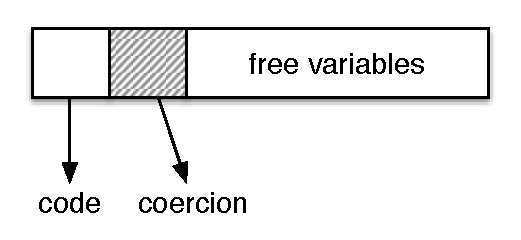
\includegraphics[width=2.5in]{closure}  
\end{center}

\footnote{\textit{Interpretations of the GTLC}. Siek \& Garcia. SFP 2012.}

}
%===============================================================================
\frame[containsverbatim]{
\frametitle{CEK Machine for the STLC}

\begin{align*}
e &::= x \mid \lam{x\of T} e \mid e \; e\\
v &::= n \mid \langle \lam{x\of T} e, \rho \rangle 
\end{align*}
\begin{align*}
\langle x, \rho, \EE \rangle & \longmapsto
    \langle \rho(x), \rho, \EE \rangle \\
\langle \lam{x\of T}e, \rho, \EE \rangle & \longmapsto
    \langle \langle \lam{x\of T}e, \rho \rangle, \rho, \EE \rangle \\
\langle (e_1 \; e_2), \rho, \EE \rangle & \longmapsto
    \langle e_1, \rho, \EE[\Hole \app \langle e_2, \rho \rangle] \rangle \\
\langle v_1, \rho, \EE[\Hole \app \langle e_2,\rho'\rangle] \rangle & \longmapsto
    \langle e_2, \rho', \EE[v_1 \app \Hole] \rangle \\
\langle v_2, \rho, \EE[\langle \lam{x\of T} e, \rho' \rangle \app \Hole] \rangle & \longmapsto
    \langle e, \rho'[x\mapsto v_2], \EE \rangle
\end{align*}

}
%===============================================================================
\frame{
\frametitle{CEK Machine for the CC}

\begin{align*}
e &::= x \mid \lam{x\of T} e \mid e \; e \mid \rd{e \CAST{c}} \\
u & ::= n \mid \langle \lam{x \of T}e, \rho, \rd{\hy{\;}{c \to d}{\;}} \rangle \mid  \\
v & ::= u \mid \rd{u \CAST{\hy{}{B}{\;!\;}}} 
\end{align*}
\begin{align*}
\langle \lam{x\of T}e, \rho, \EE \rangle & \longmapsto
    \langle \langle \lam{x\of T}e, \rho, \rd{\Id{}} \rangle, \rho, \EE \rangle \\
\langle v, \rho, \EE[\langle \lam{x\of T} e, \rho', \rd{c}\rangle \app \Hole] \rangle & \longmapsto
    \langle e, \rho'[x\mapsto v, \rd{y\mapsto c}], \EE \rangle\\
\langle e \CAST{c}, \rho, \EE \rangle & \longmapsto 
    \langle e, \rho, \EE[\Hole \CAST{c} ] \rangle \\
\langle e, \rho, \FF[\Hole \CAST{c_1}][\Hole\CAST{c_2}] \rangle & \longmapsto 
    \langle e, \rho, \FF[\Hole \CAST{c_1 \fatsemi c_2}] \rangle\\
\langle v, \rho, \FF[\Hole \CAST{c}] \rangle & \longmapsto
    \langle v', \rho, \FF \rangle 
    \quad \text{if } \mathit{coerce}(v, c) = v' \\
\langle v, \rho, \FF[\Hole \CAST{c}] \rangle & \longmapsto
    \blame{\ell} 
    \quad \text{if } \mathit{coerce}(v, c) = \blame{\ell} 
\end{align*}

}
%===============================================================================
\frame{

Apply Coercion to Value \hfill \fbox{$\mathit{coerce}(v,c) = r$}
\begin{align*}
 \mathit{coerce}(u, \hy{}{m}{\;!\;}) & = u \CAST{\hy{}{m}{\;!\;}} \\
 \mathit{coerce}(u \CAST{\hy{}{B}{\;!\;}}, c)  & = 
 \begin{cases}
   u  & \text{if } G = G' \\
   \blame{\ell} & \text{otherwise}
 \end{cases} \\
 \mathit{coerce}(\langle \lam{x} e, \rho, () \rangle, c_2) &=
   \langle \lam{y} e', \rho, c_2\rangle \\
 \text{where } e' &\equiv \Let x=y \CAST{\dom{\rho(\mathtt{c})}}
                   \In e \CAST{\rng{\rho(\mathtt{c})}} \\
 \mathit{coerce}(\langle \lam{x} e, \rho, c_1 \rangle, c_2) &=
   \langle \lam{x} e, \rho, c_1 \fatsemi c_2 \rangle \\
 \mathit{coerce}(v, \Id{}) & = v 
\end{align*}

}



% LocalWords:  titlepage containsverbatim frametitle  Siek Taha lstlisting
% LocalWords:  Rightarrow
% LocalWords:  texttt Rightarrow texttt texttt Rightarrow Findler deriv Wadler
% LocalWords:  Longrightarrow Longrightarrow circ Wrigstad ldots inc bytecode
% LocalWords:  includegraphics invokedynamic switchpoints unboxed xymatrix rrr
% LocalWords:  vspace newsavebox DistExample lrbox linewidth mathtt mathtt emph
% LocalWords:  vdash usebox mathbf mathit longmapsto mathsf subtyping emptyset
% LocalWords:  Henglein's footnotesize Drossopoulou Igarashi Gronski Dimoulas
% LocalWords:  varphi eval Jython microbenchmarks Fibonnaci vitousek bharadwaj
% LocalWords:  Shashank 
